\documentclass{cslthse-msc}
\usepackage[utf8]{inputenc}
\usepackage[english]{babel}
\usepackage{amsmath}
\usepackage{amsfonts}
\usepackage{amssymb}
\usepackage{amsthm}
\usepackage{amsmath}
\usepackage{mathtools}
%\usepackage{makeidx}
\usepackage{graphicx}
\usepackage[titletoc, header, page]{appendix}


\usepackage{hyperref}
\usepackage{pdfpages}

\usepackage{diagbox}
\usepackage{float}
\usepackage{booktabs}
\usepackage{makecell}

\DeclarePairedDelimiter\abs{\lvert}{\rvert}%
\DeclarePairedDelimiter\norm{\lVert}{\rVert}%

%\geometry{showframe}

\author{
	Christian Alexander Oliveros Labrador \\
	{\normalsize \href{mailto:christianol_01@hotmail.com}{\texttt{christianol\_01@hotmail.com}}}
	%\and
	%Camilla Lekebjer \\
	%{\normalsize \href{mailto:Camilla.Lekebjer@cs.lth.se}{\texttt{Camilla.Lekebjer@cs.lth.se}}}
}

\title{Improved Sampling \\for \\Temporal Anti-Aliasing}
\subtitle{A Sobel Improved Temporal Anti-Aliasing}
%\company{The Corporation AB LTD Inc}
\supervisor{Michael Doggett, \href{mailto:michael.doggett@cs.lth.se}{\texttt{michael.doggett@cs.lth.se}}}
%\supervisor{John Deer, \href{mailto:jdeer@company.com}{\texttt{jdeer@company.com}}}
\examiner{Flavius Gruian, \href{mailto:Flavius.Gruian@cs.lth.se}{\texttt{Flavius.Gruian@cs.lth.se}}}

\date{\today}
%\date{January 16, 2015}

\acknowledgements{
\emph{“The day we stop exploring is the day we commit ourselves to live in a stagnant world, devoid of curiosity, empty of dreams.”}
– Neil deGrasse Tyson

I have so many people to thank for this amazing adventure. Coming from Venezuela, more than 8000 km away; being the first time I am away from home for such a long time; the first time I take classes only on English; and being the first exchange student to perform a Master Thesis in the Computer Science Department at Lund University, this has been a life-changing experience. 

I would like to thank all my family, especially, my dad, Wilmer Oliveros; my mom, Raixa Labrador; and my brother, Jean Pierre Oliveros for all their help and support during this trip. Also, I would like to thank all my friends that are all over the world, thank you for helping me be who I am right now and for being with me this whole time.

I would like to thank my Lund University supervisor, Professor Michael Doggett, for giving me this amazing opportunity and for helping me through it. Also, I would like to thank Pierre Moreau for helping me whether I was stuck.
Also, I would like to thank my Universidad Simón Bolívar supervisor, Professor Angela Di Serio; and my Computer Science Coordinator, Professor Marlene Goncalves, for helping and supporting me through this incredible journey.

Finally, I would like to thank Lund University and Universidad Simón Bolívar, with special thanks to the International Office LTH; the Department of Computer Science at Lund University; the Computer Science Coordination at Universidad Simón Bolívar; and the Direction of International Relations and Cooperation at Universidad Simón Bolívar, for letting students take advantage of this type of opportunities of academic and self-growth.

\begin{figure}[!hbt]
	\centering
	
\includegraphics[scale=0.5]{images/univ_logotypes.png}
\end{figure}
}

\theabstract{
Anti-aliasing is a key component of modern 3D computer-generated imagery. For Real-Time image generation in applications such as games, it is important to increase the sampling rate per pixel to improve overall image quality. But increasing sampling can be expensive, especially for current Deferred Rendering architectures. An innovative solution to this issue is the Temporal Anti-Aliasing (TAA) technique which combines samples from previous frames with the current frame's samples to effectively increase the sampling rate. In this thesis, we will explore methods to improve the quality of TAA by using edge detection, of both color and depth, and triangle indexing to ensure only samples belonging to the current frame pixels are blending together. Our objective is to reduce ghosting and other TAA artifacts created with current implementations. Quality improvement will be evaluated by comparing TAA generated images to ground truth images generated by using much higher sample counts that would not be practical in real-time. The improved TAA was tested using image metrics, in particular, MSE, PSNR, and SSIM, against the original implementation and other current Anti-Aliasing techniques. The results obtained showed that the improvements applied to TAA enhanced the image quality above existing techniques with PSNR values around 39 and SSIM values above 0.99.
}

\keywords{TAA, Sobel, Anti-Aliasing, Triangle Indexing, TRAA}

%% Only used to display font sizes
\makeatletter
\newcommand\thefontsize[1]{{#1 \f@size pt\par}}
\makeatother
%%%%%%%%%%


\begin{document}
\makefrontmatter
\chapter[Introduction]{Introduction}
Modern Computer Graphics are based on rendering scenes that are made of objects represented as models composed of primitive polygons, the triangle being the most common one used. This is to take advantage of their simplicity and all their geometric properties to create optimal algorithms to handle their rendering. Triangles are composed of three vertices, each of them which consists of a position and other parameters associated with them, i.e. the color or normals of the triangle, for interpolation. 
 
When we want to render the objects in a scene, we take the vertices and send them to the Rendering Pipeline. There, they are processed and mapped to the pixels of the screen with their respective color.

We have two main uses for this process: Offline Applications, such as movies; and Real-time Applications, like video games. Each of them have their requirements and constraints, but for this project, we will only give attention to Real-time Applications.

The focus of this project is to improve the Temporal Anti-Aliasing algorithm, which is a technique that increases the quality of the images after the process of mapping triangles to pixels by mixing frames previously rendered with current ones.

The main requirement would be to render the highest quality possible representation of the scene, with two main constraints: we must render at least thirty frames per second, with no high frame rate loss; and we must work with a limited amount of memory and bandwidth, because we need to be able to run on an average computer or mobile device.  \cite{Doggett2017EDAN35, Shreiner2011}

\section{Problem Definition}
Temporal Anti-Aliasing (TAA) is a relatively new real-time technique that provides good results without incurring heavy memory or processing power costs of other techniques. Edge detection and triangle indexing techniques appear as good candidates to improve the quality of the technique by reducing the ghosting and blurring unwanted effects created by current implementations of TAA. 

The aim of this thesis is to improve the Temporal Anti-Aliasing technique by using edge detection, of both color and depth, and triangle indexing techniques to reduce blurring and ghosting without decreasing the quality of the rendered image or incurring in heavy memory or processing power costs.  


\section{Related Work}
As the simplest Anti-Aliasing technique, we have Super Sampling Anti-Aliasing (SSAA), it consists on rendering at a higher resolution and then downsampling it to the required resolution. Another technique is the Multi Sample Anti-Aliasing (MSAA), which calculates the color for the final pixel just once \cite{Doggett2017EDAN35}.  We can learn what would become the base of Temporal Reprojection Anti-Aliasing (TAA or TRAA) in the papers Accelerating Real-time Shading with Reverse Reprojection Caching  by Nehab D., Sander P. V., Lawrence J., Tatarchuk N., Isidoro J. R. \cite{Nehab2007}, in which they describe how pixel shaders could be used to save pixel information from the previous frame and reproject it in the next frame; and Amortized Supersampling by Yang L., Nehab D., Sander P. V., Sitthiamorn P., Lawrence J., Hoppe H. \cite{Yang2009} in which they describe how to use the reprojection of old frames in the current one as a method of real time Anti-Aliasing.

Next, we start to see Post Processing techniques like Fast Approximate Anti-Aliasing (FXAA) by Timothy Lottes \cite{Lottes2009} which uses a form of edge detection to correct aliasing while being compatible with the deferred shading architecture. We also found the Crytek implementation of Temporal Anti-Aliasing (TAA or TXAA) explained by Tiago Sousa on his presentation Anti-Aliasing Methods in CryENGINE 3 \cite{JIMENEZ2011_SIGGRAPH11}.

Enhanced Subpixel Morphological Anti-Aliasing (SMAA) by Jorge Jimenez, Jose I. Echeverria, Tiago Sousa and Diego Gutierrez \cite{Jimenez2012} which uses a more complex edge reconstruction technique while being able to work with SSAA, MSAA and a basic form of TAA.
 
Finally, we have the TRAA implementations of Ke Xu for Uncharted 4 and Lasse Fuglsang for Inside, which implement new advances like the Color Clipping Box and Sharpen Filter. These two last implementations are used as the base of this master thesis. \cite{Fuglsand2016, XU2016} 

\section{Contribution}
This thesis improves upon the last two advances from Ke Xu and Lasse Fuglsang \cite{Fuglsand2016, XU2016}. We propose the use of the Sobel Operator to perform edge detections and triangle indexing techniques to detect pixels that are considered aliased. Once we have these pixels detected, we use this information to change how colors are rejected from the past frames in order to reduce the ghosting and blurring artifacts that Temporal Anti-Aliasing has.

\chapter{Technological Background}
In this chapter, we will explain which tools were used in this master thesis and why.
\section{C++ and Bonobo Framework}
We use C++ and the Bonobo Framework to implement all of the improvements done in this Master Thesis. C++ is a compiled general-purpose programming language with imperative, object-oriented programming and low-level memory management features. We used it for its performance, especially for real-time Computer Graphics applications, and its wide knowledge base.

The Bonobo Framework is the base of the laboratories of Computer Graphics (EDAF80) and High-Performance Computer Graphics (EDAN35) courses from Lund University. It was developed in C++ and provides a rendering engine that we found easy to modify and use, especially, as the base in which we developed our improvements. 


\section{OpenGL and GLSL}
We used this Application Programming Interface (API) as it is the base of the Bonobo Framework rendering system, which we modified to develop our improvement, and because of its cross-platform compatibility. The Open Graphics Library (OpenGL) is a 2D and 3D computer cross-platform open-source graphics API that abstracts the programmer from directly interacting with the Graphics Processing Unit (GPU) to achieve hardware accelerated rendering. It provides the programmer with a graphics pipeline to use, which is normally implemented through hardware. 

We used the OpenGL Shading Language (GLSL) to implement TAA and our improvements as it is part of the OpenGL standard. GLSL is a high-level shading language that allows programmers greater control of the graphics pipeline without requiring the use of the OpenGL assembly language or hardware-specific languages.

\section{MATLAB}
We selected MATLAB to be where we developed our testing framework because of the high quality of their tools, its wide knowledge base and for its fast prototyping abilities.
MATLAB is a proprietary multi-paradigm numerical computing environment. Commonly used for science, engineering, and economics. It is popular for image processing applications because of its wide library of algorithms for this purpose, including image metrics. 

\chapter{Theoretical Background}
In this chapter, we will explain all the theoretical information that is the base of this master thesis, from the Computer Graphics Theory to the Image Metrics used.

\section{Rendering Pipeline}
Today’s graphics pipeline can be simplified into three steps: Vertex Shader, which processes the geometry associated with the vertices and prepares them for the next step; Rasterizer, which maps the triangles to pixels in the screen, calculates their visibility and interpolates the parameters of the vertices for each pixel covered by the triangle; and the Pixel (or Fragment) Shader which takes the visual pixels from the Rasterizer and colors them. Figure \ref{fig:graphpipeline} is an example of the Simplified Rendering Pipeline.

\begin{figure}[!hbt]
	\centering
	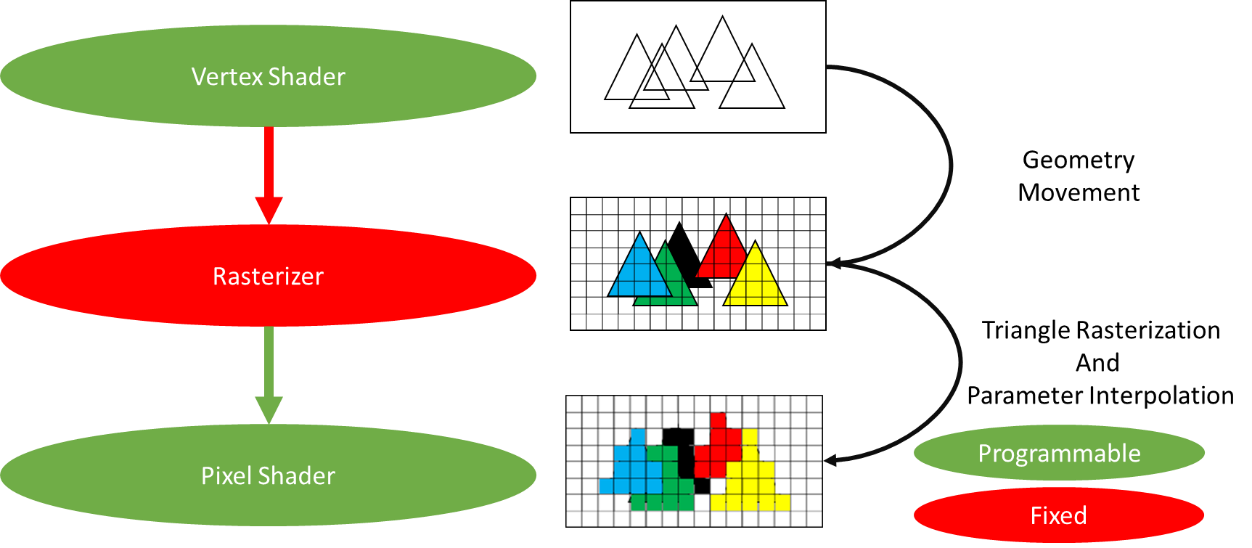
\includegraphics[scale=0.7]{images/graphics_pipeline.png} 
	\caption{Rendering Pipeline, based on EDAF80 5th Lecture.~\cite{Doggett2017EDAF80}}\label{fig:graphpipeline}
\end{figure}

It is important to note that Vertex and Pixel Shaders are controllable by a programmer using special programs called Shaders. They provide a way for the programmer to control the rendering hardware. In contrast, the Rasterizer is not controlled by the programmer and it is handled entirely by a hardware fixed function. \cite{Doggett2017EDAF80}

This Rasterization Process is important for us because it is there where some of the errors corrected by Temporal Anti-Aliasing come from.

\section{Rasterization Process}
During the Rasterization Process, each triangle is tested to establish which pixels are covered by it. While this is being done, each pixel is being tested to find out if another triangle is covering it.

In Figure \ref{fig:rasterizationproc} we have an example of the Rasterization Process. In the left image, we have the triangles as continuous surfaces before being sent to the Rasterizer and, in the right image, we have triangles mapped to the pixels on the screen after going through the Rasterizer.

\begin{figure}[!hbt]
	\centering
	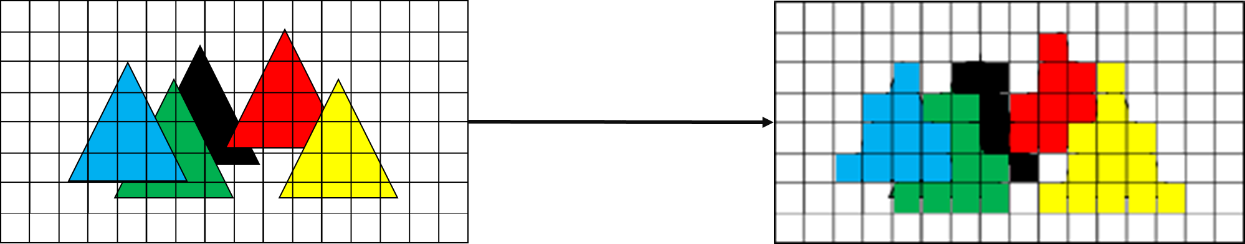
\includegraphics[scale=0.75]{images/rasterization_process.png} 
	\caption{Example of the results of the Rasterization Process. 
		\emph{Note}: colors were added to differentiate the triangles, but they would only be added at the Pixel Shader stage.
	}\label{fig:rasterizationproc}
\end{figure}

Because we are mapping a continuous triangle to a finite number of pixels, we face the problem of pixels partially covered and how to determine what is enough to qualify it as covered, Figure \ref{fig:partialcover} show examples of this problem. This is solved by calculating if the center of the pixel is covered by the triangle geometry. This process is susceptible to errors due to the precision of the representation used for the vertices.  

\begin{figure}[!hbt]
	\centering
	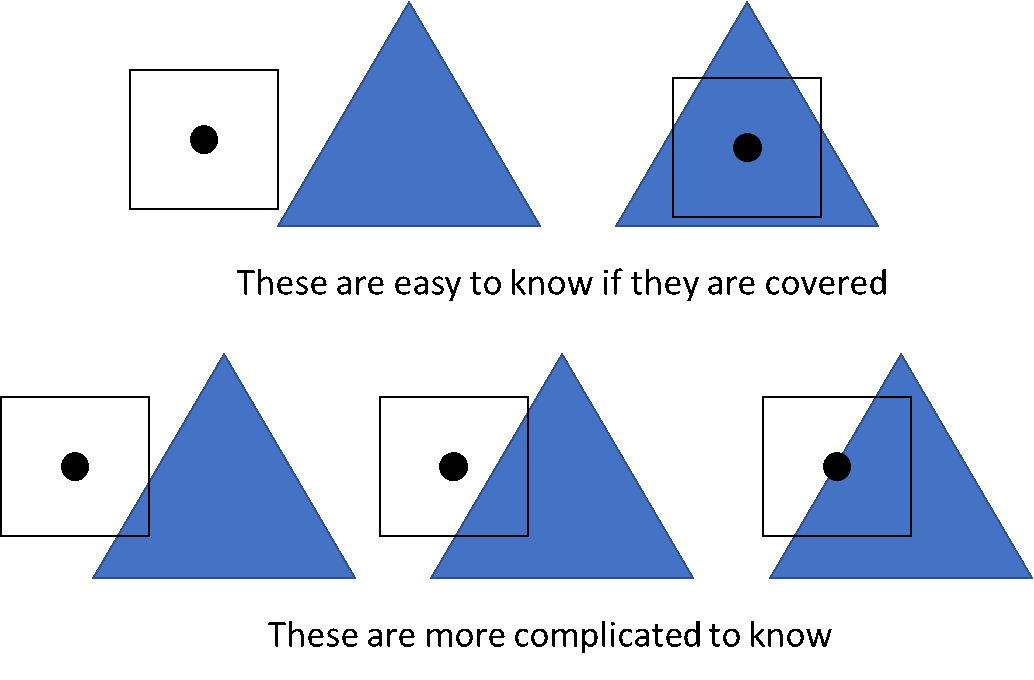
\includegraphics[scale=0.5]{images/edge_testing.png} 
	\caption{Example of the Partial Cover problem, based on EDAN35 second Lecture. ~\cite{Doggett2017EDAN35}}\label{fig:partialcover}
\end{figure}

This process shows us that what is rendered to the screen approximates what is being represented in the scene because pixels can only be covered by one triangle at a time. \cite{Moller2007, Doggett2017EDAN35}


\section{Aliasing Problem}
When we map a continuous representation to a finite one, it is going to generate errors. As explained by Edward Angel and Dave Shreiner in their book (page 413) \cite{Shreiner2011}, we can interpret the rendering process as the sampling of a continuous function $f(x, y)$, which represents the color of the scene at that point, to an $n\times m$  grid of pixels in which we assume that the point $f_{ij}$  is the value of $f$ over a small area; and to reconstruct the $f$ function to display the image to the screen using only what we know from the samples. The mathematical tool used to evaluate the issues of this process is the Fourier Analysis, which states that a function can be decomposed into a set of sinusoids, at possibly an infinite number of frequencies. For two-dimensional image analysis, we can think of the $f$ function as a set of sinusoids at two spatial frequencies.

For this thesis, we will use the First part of the Nyquist sampling theorem as a tool to illustrate why aliasing problems appear and relate to sampling problems. \\

\emph{''Nyquist Sampling Theorem (Part 1): The ideal samples of a continuous function contain all the information in the original function if and only if the continuous function is sampled at a frequency greater than twice the highest frequency in the function.}

\emph{The Nyquist frequency is defined as one half of the sampling frequency, which is the lowest frequency that cannot be in the data to avoid aliasing.''
}

Taken from Edward Angel and Dave Shreiner book page 415. \cite{Shreiner2011} \\

As Edward Angel and Dave Shreiner explain, this idealized sampling assumes that we can take an infinite number of samples per sample frequency which we cannot do in practice. The Aliasing problem that computer graphics experience comes from not being able to sample as required by the Nyquist Sampling Theorem, creating ragged edges that appear in the rasterization process (Spatial Aliasing), Figure \ref{fig:aliasingexample} shows an example of this type of aliasing, and jumps between moving objects (Temporal Aliasing), according to Doggett and Wronski  ~\cite{Doggett2017EDAN35,Wronski2014}. Many solutions have been proposed and used to solve it, e. g. the Super Sampling Anti-Aliasing (SSAA) family of solutions that work on higher frequencies than the required at the cost of more space requirements. 

\begin{figure}[!hbt]
	\centering
	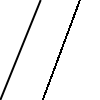
\includegraphics[scale=1.0]{images/aliasing_example.png} 
	\caption{Ground Truth image of a Line versus its Aliased Approximation.}\label{fig:aliasingexample}
\end{figure}

\section[Shadow Mapping and Deferred Shading Architecture]{Shadow Mapping and \\ Deferred Shading Architecture}

As humans, we have come to expect that objects react to the lights in a scene, considering their geometry because lights and shadows contribute with spatial information to an image, especially, shadows give us a sense of size and distance.

As explained by Doggett \cite{Doggett2017EDAN35}, under the Rendering Pipeline based on the Rasterizer, the process of shadow calculation is challenging to perform. The Rasterizer does not know if objects are covered or not from a light, so we must figure out a method to calculate if an object is in shadows. This process is called Shadow Mapping, it consists of rendering the scene through each light perspective and then perform tests against the camera perspective to establish if the object is affected by the light or if it is in shadows.

But, as we might expect, rendering the scene several times is expensive, so we need a way to reduce the cost as much as we can. The Deferred Shading Architecture provides that solution to only shade, possibly using an operation that could be expensive, only visible pixels to avoid wasting resources shading pixels from geometry that is not visible. It works by first rendering the scene, without shading calculations, to a buffer called the Geometry Buffer. There, information regarding colors, normals, depths, specific object information to interact with lights, etc. is saved for future use. 

After we have filled the Geometry Buffer, we perform the Shadow Mapping technique, which takes advantage of the Deferred Shading Architecture to calculate the way lights affects only visible pixels; we calculate the Shadow Map of every light only performing depth calculations. Afterward, we compute and save the effect of each light using the Shadow Maps. 

In the end, we take all the information of the lights, shadows, and the Geometry Buffer to render the light scene.




\section{Anti-Aliasing}
As we have explained, there are two main types of Aliasing, Spatial Aliasing, and Temporal Aliasing; Anti-Aliasing solutions provide improvements against the artifacts created by either of those types at the cost of increased rendering time. For real-time applications this increase of rendering time limits which Anti-Aliasing solutions are feasible to apply.

Another important factor that decides which Anti-Aliasing technique to use is how it behaves with current architectures. For example, old Anti-Aliasing solutions do not work with Deferred Shading.

\subsection{Super Sampling Anti-Aliasing (SSAA)}
This technique consists in rendering the scene at 4 times the size of the screen and then averaging pixels 4x4 to calculate the result \cite{Doggett2017EDAN35}. It provides good results but requires more rendering time and heavy memory usage.

\subsection{Multi Sample Anti-Aliasing (MSAA)}
MSAA consist in taking several samples per pixel; on each sample, the depth values are calculated but only one color is calculated for the rasterized triangle. This solution provides good results at the cost of increased memory usage for depth calculations. 

The biggest problem this technique has is that it does not work properly with Deferred Shading \cite{Doggett2017EDAN35}. This makes it complicated to use with current pipelines, normally requiring other corrections to reduce the artifacts created when applied with Deferred Shading.

\subsection{Fast Approximate Anti-Aliasing (FXAA)}
FXAA is a post-processing anti-aliasing technique that works by detecting edges on the rendered images and then smoothing them. \cite{Lottes2009}

It is relatively cheap compared to MSAA and provides relatively good results, its smoothing capabilities are limited by the amount of information the edge detection can get on a single pass, and it provides relatively good results for temporal aliasing.

\subsection{Enhanced Subpixel Morphological Antialiasing (SMAA)}
SMAA is a post-processing technique based on Morphological Anti-Aliasing. It works by reconstructing edges and their surroundings to regenerate the subpixel information lost by aliasing. \cite{Jimenez2012}

\section{Temporal Anti-Aliasing}
As explained by Ke Xu and Lasse Fuglsang in their respective presentations ~\cite{XU2016,Fuglsand2016}, the basic principle of Temporal Anti-Aliasing is to mix the current frame being rendered with frames from the past. This is done to increase the number of samples through time rather than only using samples from the same frame. 

One such technique is Temporal Reprojection Anti-Aliasing (TRAA), it works by saving the past frames as a History Buffer which it is then reprojected to the present scene and blended to the current frame being rendered.  To achieve this, we take the current frame and look for the color it should have in the History Buffer; this step is called Reprojection.

For TRAA to work we need to implement other common Computer Graphics techniques to serve as the base. We need Camera Jittering to be able to reconstruct pixel information around edges; a Velocity Buffer to determine the positions of the pixels on the last frame if they were moving; a Frame History Buffer to collect past frames to perform the reprojections in the next frame; a Clipping Color Box to constrain the History Buffer and avoid noise or wrong colors to appear; a Sharpen Filter to reduce part of the blur created; and Motion Blur to correct the effects of objects moving too fast for the Clipping Color Box.

\subsection{Camera Jitter}
Camera Jitter consists in moving the camera vertically and horizontally with a sub-pixel translation, Figure \ref{fig:camerajittering} is an example of the horizontal translation. It is applied every frame to preserve information from local regions of surface fragments. If the current frame is static relative to the past ones then the system is losing information that could be used to refine it. ~\cite{Fuglsand2016,XU2016}

\begin{figure}[!hbt]
	\centering
	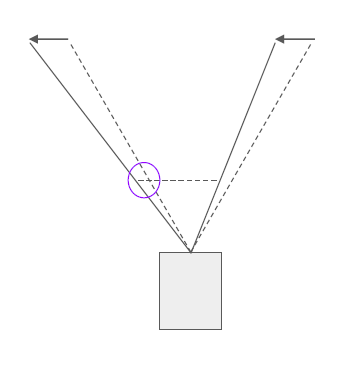
\includegraphics[scale=0.3]{images/camera_jitter.png}
	\caption{Jittering the Projection Process. Image taken from Fuglsand presentation. \protect\cite{Fuglsand2016}}\label{fig:camerajittering}
\end{figure}

The jittering is applied as a translation to the projection matrix using the $Halton Sequence (2,3)$ as translation vectors. This sequence is used because it generates an irregular pattern for the translations that help preserve more information than a regular pattern and the Halton Sequence provides a cheap pseudorandom pattern generator. ~\cite{Fuglsand2016,XU2016} 

\begin{figure}[!hbt]
	\centering
	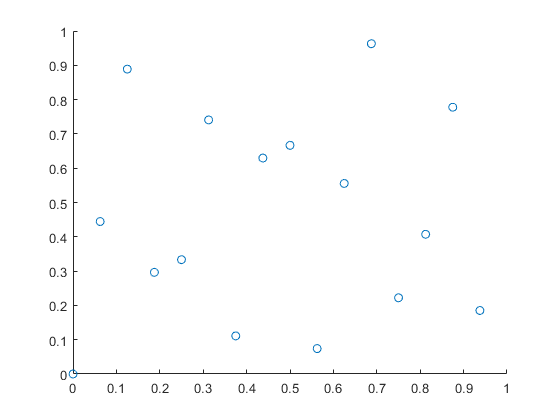
\includegraphics[scale=0.5]{images/halton_16.png}
	\caption{Values from the $Halton Sequence (2,3)$ used.}\label{fig:halton16}
\end{figure}

The Figure~\ref{fig:halton16} shows the representation of the 16 points used to jitter the projection in the current implementation, as proposed by Fuglsand ~\cite{Fuglsand2016}. The points were generated using MATLAB then scrambled to improve their randomness using reverse-radix scrambling.

\subsection{Velocity Buffer}
The Velocity Buffer algorithm used in this implementation is the one proposed by Chapman ~\cite{Chapman2012} which is calculated by subtracting the current pixel position by its last frame position. This is possible by saving the matrix that represents each object in the scene. Also, we cancel the jittering from the Camera Jittering before the calculating the velocities, to avoid the noise it creates, as suggested by Xu. ~\cite{XU2016}


\subsection{Frame History Buffer}
For each fragment in the current frame, we look for the $3\times 3$ neighborhood and plus $(+)$ pattern neighborhood (See Figure~\ref{fig:samplingpattern}). We look at both patterns for the minimum and maximum of colors of the current frame, next we average them and use them to build part of the Clipping to constrain the pixels of the History Buffer. ~\cite{Fuglsand2016}
\begin{figure}[!hbt]
	\centering
	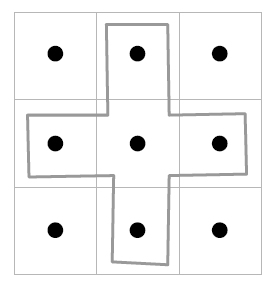
\includegraphics[scale=0.8]{images/sampling_pattern.png}
	\caption{Sampling Pattern used. Image taken from Fuglsand presentation. \protect\cite{Fuglsand2016}}\label{fig:samplingpattern}
\end{figure}

On the $3\times 3$ neighborhood we look for the velocity of the pixel with the closest depth, this is to get better edges in motion for pixels that are occluded ~\cite{Fuglsand2016}. We use this velocity to reproject the position of the current frame in the History Buffer. ~\cite{Fuglsand2016,XU2016}

After we have the pixels in the History Buffer, we constrain it (See next subsection) and linearly interpolate it with the current frame (See Figure \ref{fig:samplingprocess} for the visual representation of the complete process). We linearly interpolate both using a feedback value that is calculated by the difference of luminance between the colors of the constrained History Buffer and the current frame. This feedback value is made to bias in favor of keeping the pixel’s history over the current frame, this is done to add some information of the current frame while keeping most of the pixel's history. This linear interpolation stabilizes the image, removing the jittering and smoothing the edges ~\cite{Fuglsand2016,XU2016}. Because each pixel's history is accumulated in the History Buffer, we get the effect that pixel history from previous frames weighs less the more time the pixel's history is not rejected from the History Buffer. ~\cite{Fuglsand2016}

\begin{figure}[H]
	\centering
	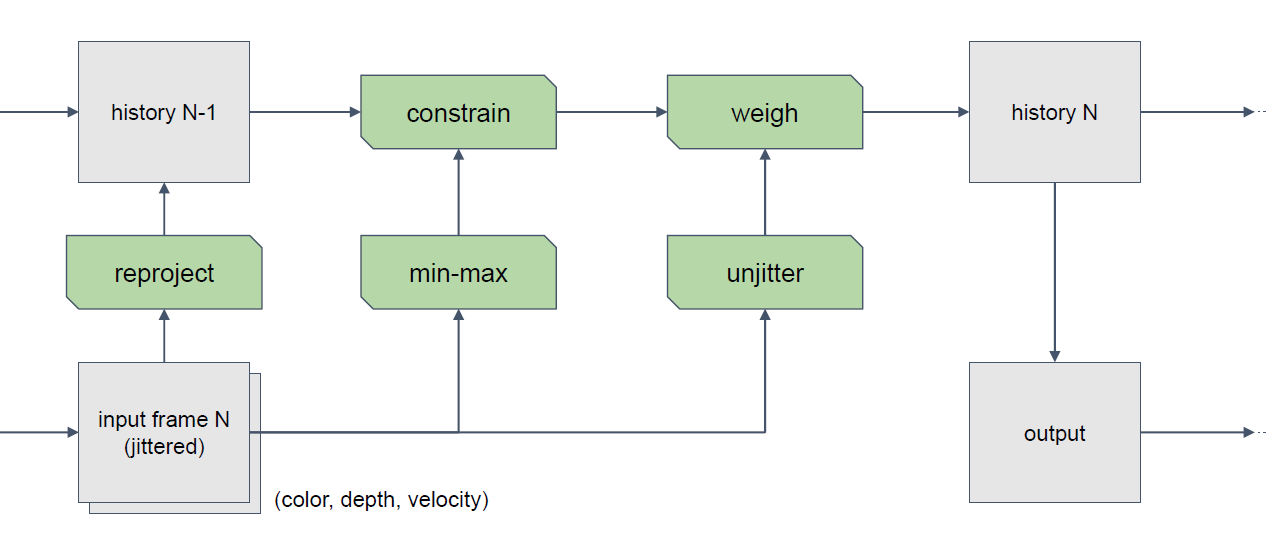
\includegraphics[scale=0.4]{images/sampling_process.png}
	\caption{Temporal Reprojection Anti-Aliasing process. Image taken from Fuglsand presentation \protect\cite{Fuglsand2016}}\label{fig:samplingprocess}
\end{figure}

\subsection{Clipping Color Box} 
A Clipping Color Box a is 3D box built using the current pixel color as the center and the minimum and maximum color calculated in the last subsection as the limits. It is used to handle color rejection when the pixel's history in the History Buffer is too distant from current color. We take the color’s history as a vector and then project it against the limits of the box; if it lies outside the projection against the border of the box is then we keep the projection, else, history’s color is left untouched. The usage of the Clipping Color Box prevents the color clustering that would happen if Clamp is applied (See Figure~\ref{fig:clippingbox}). ~\cite{Fuglsand2016}.

\begin{figure}[!hbt]
	\centering
	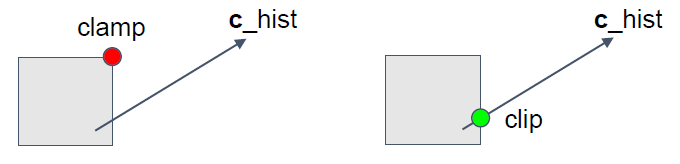
\includegraphics[scale=0.4]{images/clipping_box.png}
	\caption{Color Clamping versus Color Clipping. Image taken from Fuglsand paper. \protect\cite{Fuglsand2016}}\label{fig:clippingbox}
\end{figure}


\subsection{Sharpen Filter} 
Because the Reprojection process and Color Clipping create blurriness, a Sharpen Filter is required. We used the one proposed by Xu. ~\cite{XU2016}

\begin{equation} \label{eq:sharpen}
\begin{bmatrix*}[r]
0 & -1 &  0 \\
-1 &  5 & -1 \\
0 & -1 &  0
\end{bmatrix*}
\end{equation}

Equation \ref{eq:sharpen} being the Sharpen Filter Convolution Matrix  used in Xu paper. \protect\cite{XU2016}

\subsection{Motion Blur}
Because of the nature of the History Buffer, some ghosting is created by fragments  from objects that are moving faster than the time it takes for the Color Clipping Box to reject the color from old pixels, this is especially noticeable under special light and background conditions. Fuglsand and Xu ~\cite{Fuglsand2016,XU2016} proposed to use Motion Blur solutions to hide these artifacts.

The Motion Blur used is the one proposed by Chapman ~\cite{Chapman2012}. It tries to behave like a real camera by scaling the velocity of each pixel by the division of the current Frames Per Second (FPS) to the one wanted, thus, simulating the shutter speed. Then it mixes the colors of the pixels that are sampled while following the direction of the velocity buffer vector.


\subsection{Problems}
Temporal Anti-Aliasing has two main drawbacks, ghosting from moving objects and blurring from the way the Color Clipping Box works. This master thesis aims to help reduce the effects of these two drawbacks using new approaches but, for completeness, we present some of the current solutions available. 

\subsubsection{Blurriness} 
Current implementations of TAA generate a very aggressive blur because of the way they mix the colors of the current frame and the history; the use of areas larger than the pixel increases the errors generated, therefore a Sharpen Filter is required. The filter applied in the implementation is the one used by Xu ~\cite{XU2016}, it solves blurriness reasonably well but it cannot eliminate some artifacts. 

\subsubsection{Ghosting} 
Some Ghosting is created when objects move, especially under particular light and background conditions that make the foreground and background look alike. This is partially corrected with motion blur, nevertheless, some of it remains near objects that move fast enough to create some Ghosting but slow enough to avoid Motion Blur. Xu proposes the use of Motion Blur and to increase the size of everything using a Stencil technique and manual tagging of objects~\cite{XU2016}, but we aim to avoid requiring artists to manually tag and test objects for their ghosting behaviors. Pederson's implementation allows the jitter in the Velocity Buffer calculations to avoid ghosting but it creates some unwanted blurriness. ~\cite{Fuglsand2016}.  

\section{Accumulation Buffer}
The Accumulation Buffer is an anti-aliasing technique that consists, according to Paul Haeberli and Kurt Akeley \cite{Haeberli1990}, on rendering the scene several times with camera jittering and then performing a scaled weighted sum of the renderings to generate the current frame.

This is process increases the sampling per pixel and reduces the aliasing effects producing a high-quality image at the cost of rendering everything several times per frame.

\section{Sobel Operator}
The Sobel Operator is an efficiently computable $3\times 3$ isotropic gradient operator, as explained by Irwin Sobel \cite{Sobel2014}. We use this operator to detect edges in the rendered images to mark the as possibly aliased, because they are a common place for aliasing artifacts to appear.

It works by taking the four-possible simple central gradient estimates in a $3\times 3$ neighborhood and adding them together. The image function is taken as a density/intensity function and the four-possible estimates as orthogonal vectors which are directional derivatives multiplied by a unit vector specifying the derivative’s direction.  The sum of the four-possible simple central gradient estimates is equivalent to the vector sum of the eight directional derivative vectors.

\begin{equation}
\begin{bmatrix*}[r]\label{eq:sobel_neighborhood}
a & b & c \\
d & e & f \\
g & h & i
\end{bmatrix*}
\end{equation}

Let the Matrix \ref{eq:sobel_neighborhood} be the $3\times 3$ neighborhood and $\abs*{G}$ the magnitude of the directional derivative estimate of the neighborhood.  

The direction of $G$ will be given by the unit vector to the appropriate neighbor. Vector summing causes all the $e$ (center of the $3\times 3$ neighborhood) values to be canceled leaving only the next expression \ref{eq:sobel_simplification}:
\begin{equation}\label{eq:sobel_simplification}
\begin{split}
	G & =\frac{c-g}{4}*\begin{bmatrix*}1 & 1\end{bmatrix*}+\frac{a-i}{4}*\begin{bmatrix*}-1 & 1\end{bmatrix*}+\frac{b-h}{2}*\begin{bmatrix*}0 & 1\end{bmatrix*}+\frac{f-d}{2}*\begin{bmatrix*}1 & 0\end{bmatrix*} \\ & =\begin{bmatrix*}\frac{c-g-a+i}{4}+\frac{f-d}{2} & \frac{c-g+a-i}{4}+\frac{b-h}{2}\end{bmatrix*}
\end{split}
\end{equation}

Then we multiply by $4$ to approximate the value and ensure that we do not lose precision if we perform this with small fixed-point integers. The newly calculated magnitude is sixteen times larger than the original average gradient.

\begin{equation}\label{eq:sobel_approximation}
\begin{split}
G' = 4 * G =\begin{bmatrix*}(c-g-a+i)+(f-d)*2 & (c-g+a-i)*4+(b-h)*2\end{bmatrix*}
\end{split}
\end{equation}

Equation \ref{eq:sobel_approximation} can be expressed in two weighting matrices. We use Matrix \ref{eq:sobel_x} for the $x$ component and Matrix\ref{eq:sobel_y} for the $y$ component.

\begin{equation}
\begin{bmatrix*}[r]\label{eq:sobel_x}
-1 &  0 & +1 \\
-2 &  0 & +2 \\
-1 &  0 & +1
\end{bmatrix*}
\end{equation}

\begin{equation}
\begin{bmatrix*}[r]\label{eq:sobel_y}
+1 & +2 & +1 \\
 0 &  0 &  0 \\
-1 & -2 & -1
\end{bmatrix*}
\end{equation}

For edge-point detection, what is commonly done is compare the magnitude of $G$ against a numeric threshold to mark points as edges. 

\section{Image Metrics}
The process of measuring the quality of an image is a complicated one. As explained by Al-Najjar and Soong \cite{Yusra2012}, we can follow two main methods: subjective or objective. The subjective methods are based on opinions collected from humans and, as one would expect, are considered expensive, difficult to implement and time-consuming to perform. The second kind of methods, the objective ones, are based on mathematical formulas and algorithms to measure the quality of the image without human intervention. For this thesis, we are using objective methods. 

Objectives methods can be categorized into three groups, as described by Al-Najjar and Soong \cite{Yusra2012}:

\begin{itemize}
	\item \textbf{No-Reference:} In which we have no reference image to compare with.
	\item \textbf{Reduced-Reference:} Where we have part of a reference image.
	\item \textbf{Full-Reference:} We have the complete reference image.
\end{itemize}

For computer graphics, the preferred methods are the Full-Reference ones because reference images can be generated using higher quality but bad performing algorithms to render them. The most common metrics used, and the ones used in this thesis, are: Mean Square Error (MSE); Peak Signal-to-Noise Ratio (PSNR); and the Structural Similarity Index (SSIM).

\subsection{Mean Square Error (MSE)}
Based on the average of the squared error between the pixels of the image and the reference.

\begin{equation}\label{eq:mse}
	MSE=\frac{1}{N*M}\sum\limits_{i=0}^{N-1}\sum\limits_{j=0}^{M-1}(Im(i,j)-Ref(i,j))^2
\end{equation}
Where $N,M$ are the width and height of the images and $Im,Ref$ are the pixel of the Image and Reference.

\subsection{Root Mean Square Deviation (RMSD)}
It is the standard deviation of MSE. Also called Root Mean Square Error (RMSE).
\begin{equation}\label{eq:rmse}
RMSE=\sqrt{MSE}
\end{equation}

\subsection{Peak Signal-to-Noise Ratio (PSNR)}
It is based on the mathematical concept of Signal-To-Noise Ratio (SNR) which measures the signal of the image, which is stored as the colors of the pixels for our purposes, against its error compared to the reference. \cite{Yusra2012}

\begin{equation}\label{eq:psnr}
PSNR=10*\log\left(\frac{S^2}{MSE}\right)
\end{equation}

Where $S$ is the maximum value the signal can achieve.In our case it is $255$ because we use 8-bit color channels. 

\subsection{Structural Similarity Index (SSIM)}
SSIM is a widely used image metric that matches human subjectivity and is highly sensitive to degradations in the spatial structure of image luminance, as explained by Malpica and Bovik. \cite{Malpica2009}

It requires two images to compare, $X$ and $Y$, and three similarity functions are performed in a sliding $N\times N$ (typically $11\times 11$) gaussian weighted window.

\begin{equation}\label{eq:ssim_components}
\begin{split}
l(x,y) & = \frac{2*\mu_X(x,y)*\mu_Y(x,y)+C_1}{\mu_X^2(x,y)+\mu_Y^2(x,y)+C_1} \\ 
c(x,y) & = \frac{2*\sigma_X(x,y)*\sigma_Y(x,y)+C_2}{\sigma_X^2(x,y)+\sigma_Y^2(x,y)+C_2} \\ 
s(x,y) & = \frac{\sigma_{XY}(x,y)+C_3}{\sigma_X(x,y)+\sigma_Y(x,y)+C_3}
\end{split}
\end{equation}

Where
\begin{equation*}
\begin{split}
\mu_X(x,y) & = \sum\limits_{p=-P}^{P} \sum\limits_{q=-Q}^{Q} w(p,q)*X(x+p,y+q)\\ 
\sigma_X^2(x,y) & = \sum\limits_{p=-P}^{P} \sum\limits_{q=-Q}^{Q} w(p,q)*\lbrack X(x+p,y+q)-\mu_X(x,y) \rbrack^2\\ 
\sigma_{XY}(x,y) & = \begin{split}\sum\limits_{p=-P}^{P} \sum\limits_{q=-Q}^{Q} w(p,q)& *\lbrack X(x+p,y+q)-\mu_X(x,y)\rbrack \\ & *\lbrack Y(x+p,y+q)-\mu_Y(x,y)\rbrack\end{split}
\end{split}
\end{equation*}

Where $w(p,q)$ is a Gaussian weighing function such that $\sum\limits_{p=-P}^{P} \sum\limits_{q=-Q}^{Q} w(p,q)=1$ and $C_1,C_2,C_3$ are small constants that provide stability when the denominator approaches zero. Typically, they are set as follows: 
\begin{equation*}
	C_1=(K_1*L)^2,C_2=(K_1*L)^2,C_3=\frac{C_2}{2}
\end{equation*}

Where L is the dynamic range of the image and $K_1,K_2\ll1$ are small constants. At the end, the three similarity functions are combined in the general form: 

\begin{equation}\label{eq:ssim}
SSIM(x,y)=l(x,y)*c(x,y)*s(x,y)
\end{equation}



\chapter{Development}
In this chapter, the main work performed in this master thesis is presented.
\section{EDAN35 Project Improvements}
For this master thesis, we decided to use our project from High Performance Computer Graphics (EDAN35) as the base. During the course, we implemented a Temporal Reprojection Anti-Aliasing technique based on the presentations of Ke Xu and Lasse Fuglsang ~\cite{XU2016,Fuglsand2016}, from the games Inside and Uncharted 4. It proved to be reliable and well documented; and allowed us to put into practice the fundamentals of the technique in an academic environment, providing the base for improvements performed for this master thesis.

The EDAN35 project implementation had errors in the jittering process that were corrected by properly expanding what both implementations meant by camera jittering , see Appendix \ref{appendix:jitter} for a full explanation. The management of the Halton points was redone to accomplish the improved camera jittering with the inclusion of support of up to 128 points to work as the jittering of the Accumulation Buffer (See Figure \ref{fig:halton128}). Note, though, for Temporal Anti-Aliasing only the first 16 points are used as suggested by Xu and Fuglsang. ~\cite{XU2016,Fuglsand2016}

\begin{figure}[!hbt]
	\centering
	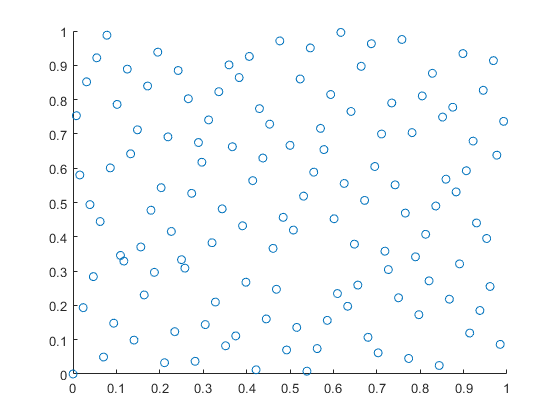
\includegraphics[scale=0.5]{images/halton_128.png}
	\caption{The $128$ $Halton Sequence (2,3)$ points available to use.}\label{fig:halton128}
\end{figure}

Specular Lighting Anti-Aliasing is a complex problem by itself, which requires specialized solutions that work directly with light reflections. Anti-Aliasing techniques do not correct it by themselves, they usually work with suitable already made solutions. To avoid problems with Specular Lighting, it was decided to be turned off.

Also, there were added models for a sphere, wall, pipe, hairball, a window with blinds and an arched window to test the improvements done to the Temporal Anti-Aliasing. All models, except the wall, were added with one color-solid texture to avoid introducing lighting errors in the calculations of the image metrics for the comparisons between the Uncharted 4 implementation and the one developed in this master thesis. The wall model uses a white texture with black letters on it because letters use hard edges to define their shape and must stay that way after applying any Anti-Aliasing technique.

\subsection{Fast Approximate Anti-Aliasing (FXAA)}
For this master thesis, the white paper version of Fast Approximate Anti-Aliasing (FXAA) by Lottes \cite{Lottes2009} was used to compare it against Temporal Anti-Aliasing, on the ground that both techniques are Post-Processing Anti-Aliasing and that FXAA is a popular technique used in the industry. It was implemented  under the highest quality preset according to the white paper without taking into consideration the performance impact because we wanted to compare the raw improvement that both techniques can provide.

\subsection{Enhanced Subpixel Morphological Antialiasing (SMAA)}
In order to test a more complex and newer post-processing technique, SMAA was implemented following the instructions provided by Jimenez et al. \cite{Jimenez2012}. It was implemented using the highest     preset that works with the deferred shading pipeline.

\subsection{Accumulation Buffer}
We use an Accumulation Buffer to provide a reference image of what the scene is. It was implemented following Haeberli and Akeley \cite{Haeberli1990}. The points used to jitter the camera are Halton Sequence Points as for Temporal Anti-Aliasing, although the Accumulation Buffer can use up to 128. The reasons for using Halton Sequence are that: it fulfils the requirements established by Haeberli and Akeley; it is easy to extend the current camera system to support more Halton Points; and for Temporal Anti-Aliasing, it provides pseudo-random points that do not follow a pattern to help gather as much information of the scene as possible.

\subsubsection{Sample Number Selection}
The number of samples selected for the Accumulation Buffer is 128. This is because it provides the best representation possible of the scene even though it causes a substantial loss of performance.

In order to show the difference between using 16 and 128 samples, we performed four tests, named from A to D, to observe how the metrics behave under different arrangements  of scene objects and lighting. In the Table \ref{tab:acctest} we see the results of one such test:

\begin{table}[!hbt]
	\centering
	\caption{Metrics behavior comparison between using 16 samples versus 128 for Accumulation Buffer.}\label{tab:acctest}
\begin{tabular}{ | l | c | c | c | c | }
	\hline
	\multicolumn{5}{| c |}{\textbf{Test D}} \\
	\hline
	\textbf{\diagbox{Tests}{Samples}}  & \textbf{\makebox{16}} & \textbf{\makebox{128}} & \textbf{\makebox{Difference}} & \textbf{\makebox{Relative Difference $(\%)$}} \\
	\hline
	MSE of Temporal	& $40.647863$ & $38.947297$	& $-1.700566$ & $4.183654132\%$ \\
	\hline
	RMSD of Temporal & $6.375568$ & $6.240777$ & $-0.134791$ & $2.114180258\%$ \\
	\hline
	MSE of No AA & $24.872104$ & $24.524992$ & $-0.347112$ & $1.395587603\%$ \\
	\hline
	RMSD of No AA & $4.987194$ & $4.952271$ & $-0.034923$ & $0.700253489\%$ \\
	\hline
	Peak-SNR of Temporal & $32.040426$ & $32.22603$ & $0.185604$ & $0.575944353\%$ \\
	\hline
	SNR of Temporal & $30.30596$ & $30.492374$ & $0.186414$ & $0.611346299\%$ \\
	\hline
	Peak-SNR of No AA & $34.173678$ & $34.234715$ & $0.061037$ & $0.178289786\%$ \\
	\hline
	SNR of No AA & $32.439212$ & $32.501058$ & $0.061846$ & $0.190289190\%$ \\
	\hline
	SSIM of Temporal & $0.993302$ & $0.993451$ & $0.000149$ & $0.014998223\%$ \\
	\hline
	SSIM of No AA & $0.996826$ & $0.996891$ & $6.5E-05$ & $0.006520272\%$ \\
	\hline		
\end{tabular}
\end{table}

The changes are large enough on some metrics to be noticeable, especially on MSE and SSIM of Temporal Anti-Aliasing, for our comparisons between Anti-Aliasing techniques. We are going to notice the effects of the use of 128 samples when we reach the comparisons between Anti-Aliasing techniques.

\section{Testing Framework Implementation}
To measure any improvement achieved, we developed a testing framework that allows us to save the important information when the test is performed. The framework allows us to select which technique to use as the main renderer: the Master Thesis Temporal Anti-Aliasing implementation; Uncharted 4 Temporal Anti-aliasing implementation; Enhanced Subpixel Morphological Antialiasing (SMAA); or Fast Approximate Anti-Aliasing (FXAA). It also allows us to zoom any part of the screen and then perform all the image metrics calculations using MATLAB.

When a test is performed, selected rendered images are saved as PNGs with 4 color channels and no compression. Also, basic information regarding the date when the test was performed; the camera information and data regarding the values used for Temporal Anti-Aliasing are saved in a plain text file.
To quantify if improvements were achieved on the main objectives of this thesis, ghosting, and blurriness, two different types of tests were developed: Static Test and Ghosting Test.

\subsection{Static Test}
This type of test consists of letting the History Buffer fill for 16 frames by rendering the scene without any moving object with the Temporal Anti-Aliasing technique selected and then saving the last frame rendered. Immediately after saving the last TAA frame rendered, we render the last frame again but now using the Accumulation Buffer, to generate the ground truth image of the scene, and SMAA, FXAA and No Anti-Aliasing (No AA), for comparison purposes. 

\subsection{Ghosting Test}
This type of test is performed only with the sphere and hairball models; the first is moving through the alley of the scene simulating a moving object in an application and the second one is rotating in a static position simulating many edges moving. The test consists of rendering the scene for a selected number of frames, with the Master Thesis Temporal Anti-Aliasing implementation and the Uncharted 4 Temporal Anti-Aliasing implementation at the same time. After each frame is rendered, each image, the position of the sphere and the rotation of the hairball are saved.

Once the selected number of frames has run through, the sphere is returned to its original position and the movement is repeated using the positions saved before; and the hairball is returned to its original rotation and the movement is also repeated. The difference this time is that every frame is rendered using the Accumulation Buffer and then saved, it is done to avoid the heavy performance loss caused by the Accumulation Buffer impacting the Temporal Anti-Aliasing techniques.

After all the images rendered are saved, we compare the ones produced by the Master Thesis Temporal Anti-Aliasing and the Uncharted Temporal Anti-Aliasing against the ground truth to calculate the image metrics of them. The image metrics we calculate show how much error was generated by ghosting in both implementations, allowing us to compare how both techniques behave. 


\subsection{MATLAB Image Metrics}
The images metrics for each test represent, numerically, the quality of each image. We calculate them to compare how each technique behaved on each test in order to identify if the Master Thesis Temporal Anti-Aliasing generates higher quality images than the other techniques tested. 

Once all the test results are saved, one script takes all the images and organizes them into folders by name and type of test. Afterward, all the test results are processed using MATLAB to get the images metrics results. With the image metrics results, we compare how the Mater Thesis Temporal Anti-Aliasing behaved against the Uncharted 4 Temporal Anti-Aliasing and the other Anti-Aliasing techniques, to detect if the improvements worked and to observe how our improved implementation behaved against other common Anti-Aliasing techniques.

For Static Tests, we perform MSE, RMSD, PSNR, SNR and SSIM measurements to the TAA, FXAA, SMAA and No AA rendered images, using the Accumulation Buffer rendered images as the reference to compare with. Also, we generate a local SSIM map for each rendered image, apart from the one rendered with the Accumulation Buffer, which are saved as PNGs and MATLAB FIGs. All the measurements results are stored in the folder with the test results as plain text. 

For Ghosting Tests, we perform MSE, RMSD, PSNR, SNR and SSIM measurements to each frame rendered with the Temporal Anti-Aliasing of Uncharted 4 technique and the Temporal Anti-Aliasing of the Master Thesis using the corresponding Accumulation Buffer rendered frame. A local SSIM map is generated for each rendered image, except the Accumulation Buffer ones, and saved as PNGs and MATLAB FIGs. All the results of all images are stored in a plain text file. In the SSIM maps, dissimilarity is represented as colors and white as similarity.


\section[Temporal Reprojection Anti-Aliasing Modifications]{Temporal Reprojection \\ Anti-Aliasing Modifications}
For this thesis, the Color Clipping Box technique was modified to be affected by the values calculated from the new techniques applied in this thesis. These changes follow the rationale that we want to apply the full force of the Temporal Anti-Aliasing technique when needed, and not elsewhere, to minimize the effects of ghosting and blurring.

The first change consists in that the Colors that were calculated from the average between the $3\times 3$ and Cross neighborhoods by the sampling patterns (See Figure \ref{fig:samplingpattern_2}) are now mixed in a variable amount. This follows the idea that we prefer the Cross neighborhood if the pixel we are currently calculating is not considered to be aliased because the Cross neighborhood is less likely to introduce noise in the Color Clipping Box calculations. But, if the pixel is considered to be aliased, we prefer the $3\times 3$ neighborhood because it provides more information about the surroundings of the pixel to create the unaliased image.  

\begin{figure}[!hbt]
	\centering
	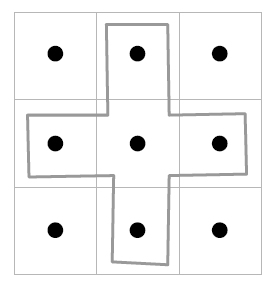
\includegraphics[scale=0.3]{images/sampling_pattern.png}
	\caption{Sampling Pattern used. Image taken from Fuglsand presentation. \protect\cite{Fuglsand2016}}\label{fig:samplingpattern_2}
\end{figure}

The second change is that the size of the Color Clipping Box depends on how much the pixel is considered to be aliased. By using smaller Color Clipping boxes (See Figure \ref{fig:colorclippingboxredux}) than the original technique on unaliased pixels, we increase the elimination of unwanted colors from the history, reducing the effects of ghosting since we are rejecting colors faster on pixels that we know are not considered to be aliased. This is implemented by linearly interpolating the current pixel color and the minimum and maximum colors calculated for the Color Clipping Box.

\begin{figure}[!hbt]
	\centering
	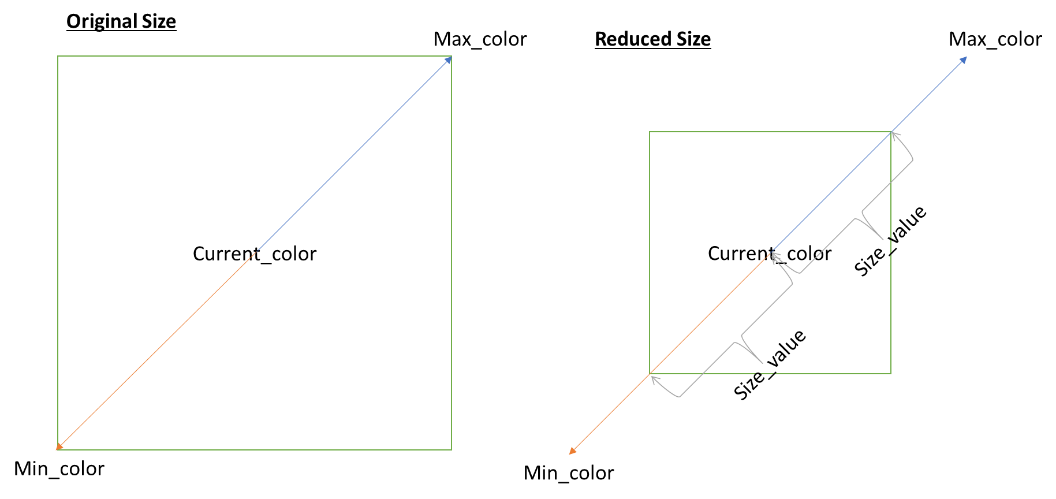
\includegraphics[scale=0.7]{images/clipping_box_reduction.png}
	\caption{Color Clipping Box size reduction}\label{fig:colorclippingboxredux}
\end{figure}

On the next subsections, we explain how all the values are calculated that contribute to decide if a pixel is considered aliased or not. All of these values are calculated at the same time as TAA is being applied, with the exception of the Sobel Operator which happens before the main TAA technique. Afterward, we show how we use that value to reduce the size of the Color Clipping Box and the preference of the Sampling Pattern.

\subsection{Triangle Indexing Improvements Implementation}
The main idea behind the application of this technique is to detect pixels that we considered aliasing by using the number of different models the pixel is surrounded with. We want to detect the edges between different models because aliasing normally occurs there. Once we have this information, we proceed to alter the Color Clipping Box that controls the application of TAA.

To implement this technique, all models in the scene receive a unique integer index. Then, in the renderization geometry pass, all triangles belonging to the same model receive the model index as its ID. Subsequently, it is used in the pixel shader to generate a texture in which every pixel contains the ID of the model it belongs to.

On the Temporal Reprojection pass, the average on the number of pixels belonging to different models in the $3\times 3$ neighborhood of the current pixel is calculated. With this average, we proceed to skew the color linear interpolation between the minimum, maximum and average between the Cross and $3\times 3$ neighborhoods of the pixel and we proceed to change the size of the Color Clipping Box. 

If the average is close to zero, meaning that the pixel is surrounded by pixels of its same model, we interpolate towards colors from the Cross neighborhood and reduce the size of the Color Clipping Box. But, if the average is close to one, meaning that the pixel is surrounded by many pixels of other models, we interpolate towards colors from the $3\times 3$ neighborhood and let the Color Clipping Box stay on its original size.

\begin{equation}\label{eq:model_index_acc}
modelAverage_i = \frac{\sum\limits_{j=1}^{9} ModelDiff(i,j)}{9} 
\end{equation}

Where
\begin{equation*}
ModelDiff(i,j) = \left\lbrace \begin{split}1\quad & if\quad ModelID_i \neq ModelID_j \\ 0\quad & else\end{split} \right.
\end{equation*}

Next we are going to show some examples of how this technique works. For each matrix, the numbers represent the triangles ID's with the center position being the current pixel being calculated and the rest being its neighborhood. Matrix \ref{eq:triang_index_not_aliased} shows an example of a pixel not considered aliased because most of the neighborhood have the same ID. On the other hand, Matrix \ref{eq:triang_index_aliased} shows a pixel considered aliased because of the high amount of different ID's around.

\begin{equation}
\begin{bmatrix*}[r]\label{eq:triang_index_not_aliased}
3 &  3 & 3 \\
3 &  3 & 3 \\
5 &  23 & 82
\end{bmatrix*}
\end{equation}

\begin{equation}
\begin{bmatrix*}[r]\label{eq:triang_index_aliased}
3 &  3 & 3 \\
3 &  5 & 3 \\
5 &  23 & 82
\end{bmatrix*}
\end{equation}

\subsection{Depth Pseudo-Variance and Depth Temporal Pseudo-Variance}
The key point behind this technique is that we want to detect pixels that we consider aliased because they are in a neighborhood of pixels separated by relatively long depth distances or that their depth in the last frame changed relatively a long distance in contrast to its current neighborhood.

First, we calculate the minimum, maximum and average linear depth from the $3\times 3$ neighborhood. Then we proceed to use the next formula to calculate the value we are going to use to normalize results:
\begin{equation} \label{eq:maxdepthdistance}
\begin{split} 
	maxDepthDistance = min \left( \right. & \left| depthMin-depthAvg \right|  ,   \\ 
	 &  \left.\left| depthMax-depthAvg\right| \right) 
\end{split} 
\end{equation}

We calculate the normalizing value using the minimum to avoid the interference of outliers. If $maxDepthDistance$  is below $0.002$ everything that follows is set to zero because pixels are so close that it is probably not aliased. This threshold was defined by experimenting which values would not get noise inside the calculations but would let the interesting pixels in. 

Then we calculate the depth pseudo variance as:

\begin{equation} \label{eq:depthpseudovariance}
	depthPseudoVariance = \left( \frac{\left|currentDepth-depthAvg\right|}{maxDepthDistance}\right)^2
\end{equation}

This provides us with a pseudo-variance that measures the distance between the average depth and the current pixel depth. Note that normally the value is going to be between $0$ and $1$ and but, if the pixel depth is an outlier, this value is going to be over $1$.

Finally, we calculate how the depth of the pixel in the last frame relates to the current neighborhood, using the depth temporal pseudo variance. Note that we use the fourth power to reduce the noise in the calculations because the normalized value is between $0$ and $1$, therefore, making it converge to $0$ if the value was near $0$.

\begin{equation} \label{eq:depthtemporalpseudovariance}
depthTemporalPseudoVariance = \left( \frac{\left|pastDepth-depthAvg\right|}{maxDepthDistance}\right)^4
\end{equation}

Next, we are going to show examples of how this technique decides if a pixel is considered aliased or not. For each matrix, the numbers represent the triangles depths with the center position being the current pixel being analyzed and the rest being its neighborhood.  Matrix \ref{eq:depth_var_not_aliased} shows us an example of a pixel not considered aliased because it is relatively close to most of its neighborhoods. In contrast, Matrix \ref{eq:depth_var_aliased} shows an example of a pixel that would be considered aliased because it has a relatively big distance in comparison to its neighborhood. An example of a pixel considered aliased by the Depth Temporal Pseudo-Variance would be if the depth of the pixel of Matrix  \ref{eq:depth_var_not_aliased} in the last frame was $4.0$.

\begin{equation}\label{eq:depth_var_not_aliased}
\begin{bmatrix*}[r]
9.0 &  9.3 & 8.7 \\
9.2 &  9.0 & 9.3 \\
8.8 &  8.9 & 8.7
\end{bmatrix*}
\end{equation}

\begin{equation}\label{eq:depth_var_aliased}
\begin{bmatrix*}[r]
9.0 &  9.3 & 8.7 \\
9.2 &  4.0 & 9.3 \\
8.8 &  8.9 & 8.7
\end{bmatrix*}
\end{equation}

\subsection{Sobel Improvements Implementation}
The main idea behind applying Sobel edge detection technique is to concentrate the TAA effects on pixels on edges to correct aliasing, if necessary.  It is important to note that this is the only technique from the improvements of the master thesis that runs before the main TAA algorithm.

We apply the Sobel Operator to the luminance of the colors of the lit scene produced by the Deferred Shading Pipeline, the luminance of the colors of the unlit scene from the Geometric Buffer, and the current linear depth. We use luminance because the human eye is better at recognizing sudden changes on it and we use the lit and unlit scene to avoid problems detecting edges because of lights or shadows. 

Each Sobel Operator is performed separately, and their magnitudes mixed at the end as follows:
\begin{equation} \label{eq:sobel_g}
	g=(u*0.3 +l*0.7)+d 
\end{equation}

Where $u$ is the magnitude of the sobel operator of the luminance of the unlight scene, $l$ is the magnitude of the sobel operator of the luminance of the lighted scene and $d$ is the magnitude of the sobel operator of the current linear depth. \\

Then, we clamp $g$ between $0.0$ and $1.0$ to finally apply the smoothstep polynomial as follows:
\begin{equation} \label{eq:sobel_sqrt}
sobel=\sqrt{g^2*(3.0-2.0*g)} 
\end{equation}

After all the Sobel Operators are applied, we save the results to a texture and perform a simplified version of TRAA to keep the results stable through time. This simplified version is almost the same as the one we use as a base of this master thesis, the differences come from the use of Clamping rather than a Clipping Box because the texture values are one dimensional; and we do not apply a sharpen filter.

The output of this TRAA is used to calculate the Sobel value of the current pixel, the average Sobel value in the Cross Neighborhood and the average Sobel value in the $3\times 3$ Neighborhood.

\subsection{Final Mixing}
Finally, we  modify how the Clipping Box is calculated using the values we previously calculated. We call this final mixed value $aliasedValue$, it represents how much a pixel is considered to be aliased. After it is calculated, we use it to change the Sampling Pattern from which colors the Color Clipping Box is built upon and its  size.

First , we define the mix function as follows:
\begin{equation} \label{eq:mixfunction}
Mix(x,y,t)=x*(1-t)+y*t\quad with\; 0\leq t\leq 1
\end{equation} 

Then, the final mixing is applied as follows:
\begin{equation}\label{eq:sobelavgmixval}
sobelAvgMixVal=Clamp01(modelAverage_i+sobel) 
\end{equation}
 
Where $sobel$ is the Sobel value of the current pixel, Equation \ref{eq:sobel_sqrt}, $modelAverage_i$ comes from the Equation \ref{eq:model_index_acc} and $Clamp01$ is the clamping function between $0$ and $1$. \\

\begin{equation}\label{eq:sobelavg}
sobelAvg=Mix(sobelAvgCross, sobelAvg3x3, sobelAvgMixVal)
\end{equation}

Where $sobelAvgCross$ is the average Sobel value of the Cross Neighborhood and $sobelAvg3x3$ is the average Sobel value of the $3\times 3$ Neighborhood around the current pixel. \\ 

And, we use Equations \ref{eq:sobelavg}, \ref{eq:depthpseudovariance}, \ref{eq:depthtemporalpseudovariance} and \ref{eq:model_index_acc} to calculate how much this pixel is considered to be aliased:
\begin{equation}\label{eq:aliasedvalue}
\begin{split}
aliasedValue=Clamp01 (& sobelAvg + depthPseudoVariance \\
 & + depthTemporalPseudoVariance \\
 & + modelAverage_i)
\end{split}
\end{equation}

With this $aliasedValue$ we proceed to modify the Color Clipping Box. First, we select how much of each Sampling Pattern we want to be part of the Color Clipping Box:
\begin{equation}\label{eq:newcolors}
\begin{split}
colorMin= & Mix(colorMinCross,colorMin3x3,aliasedValue) \\
colorMax= & Mix(colorMaxCross,colorMax3x3,aliasedValue) \\
colorAvg= & Mix(colorAvgCross,colorAvg3x3,aliasedValue) \\
\end{split}
\end{equation}

Then we modify the size of the Color Clipping Box by interpolating towards the normal size if the $aliasedValue$ is close to one, else, we use the current color, which is the center of the box.
\begin{equation}\label{eq:clipredux}
\begin{split}
	clipColorMin= & Mix(colorCurrent,colorMin,aliasedValue) \\
	clipColorMax= & Mix(colorCurrent,colorMax,aliasedValue)
\end{split}
\end{equation}



The Figures \ref{fig:aliasedval1}, \ref{fig:aliasedval2} and \ref{fig:aliasedval3} are examples of the aliased values calculated, each pixel is the current $aliasedValue$ of that picture. The white color represents an $aliasedValue$ of $1$ and the black color of $0$. As we expect, most the edges are marked as probably aliased by the techniques we used.

\begin{figure}[H]
	\centering
	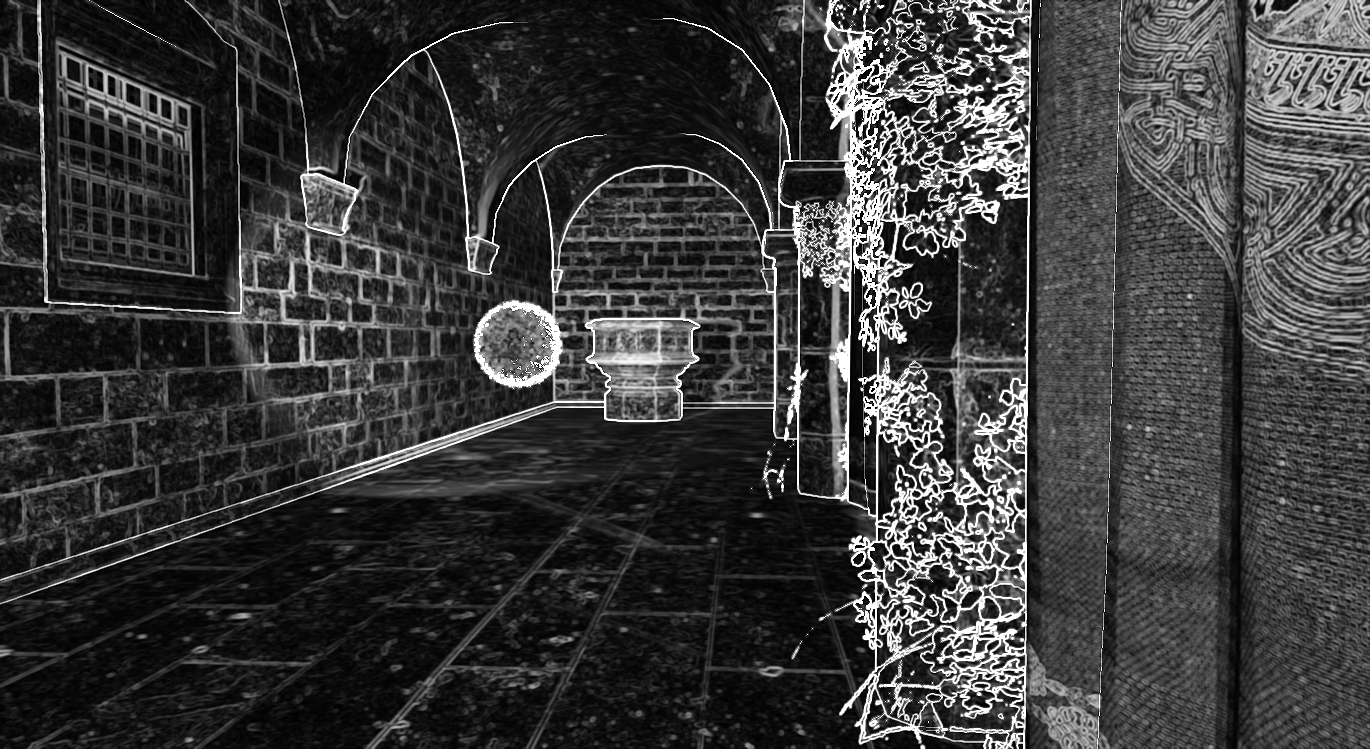
\includegraphics[scale=0.2]{images/aliased_value_example_1_temporal.png}
	\caption{Image made of the Aliased Values of each pixel.}\label{fig:aliasedval1}
\end{figure}

\begin{figure}[H]
	\centering
	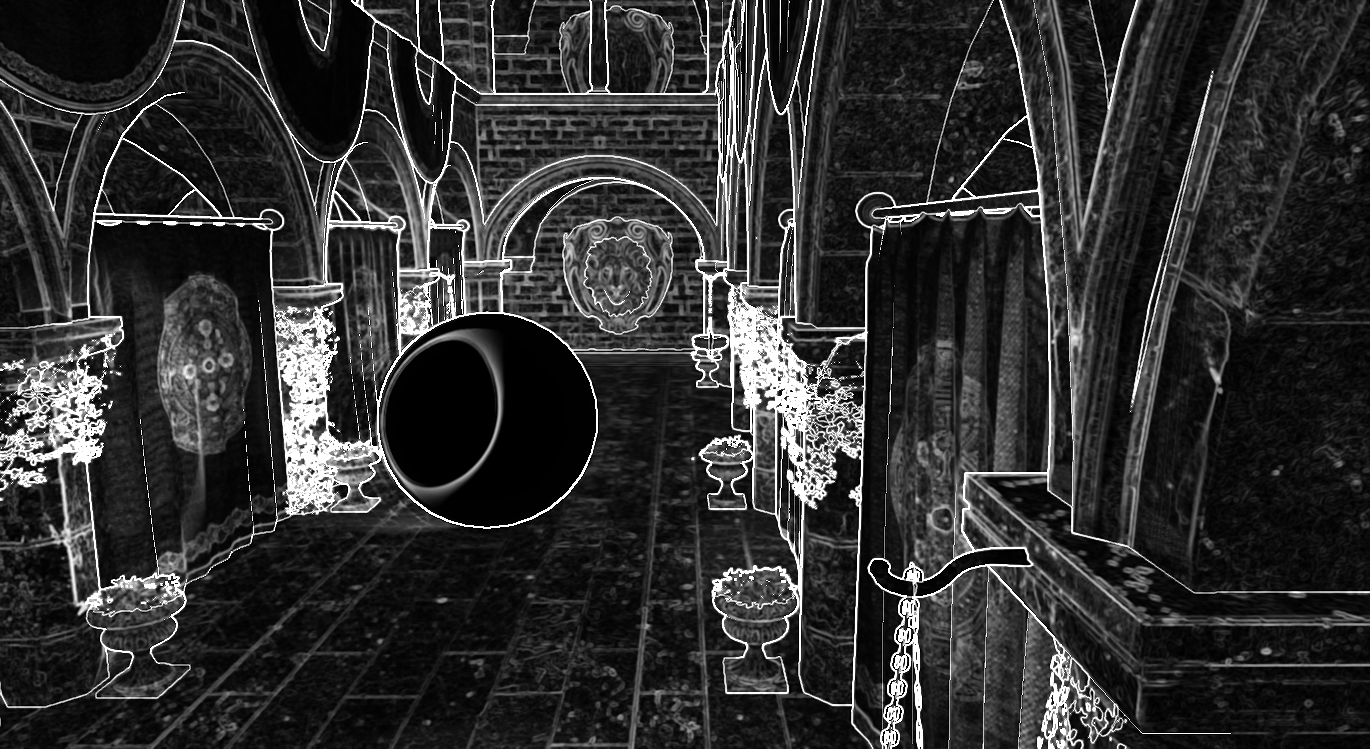
\includegraphics[scale=0.2]{images/aliased_value_example_2_temporal.png}
	\caption{Image made of the Aliased Values of each pixel.}\label{fig:aliasedval2}
\end{figure}

\begin{figure}[H]
	\centering
	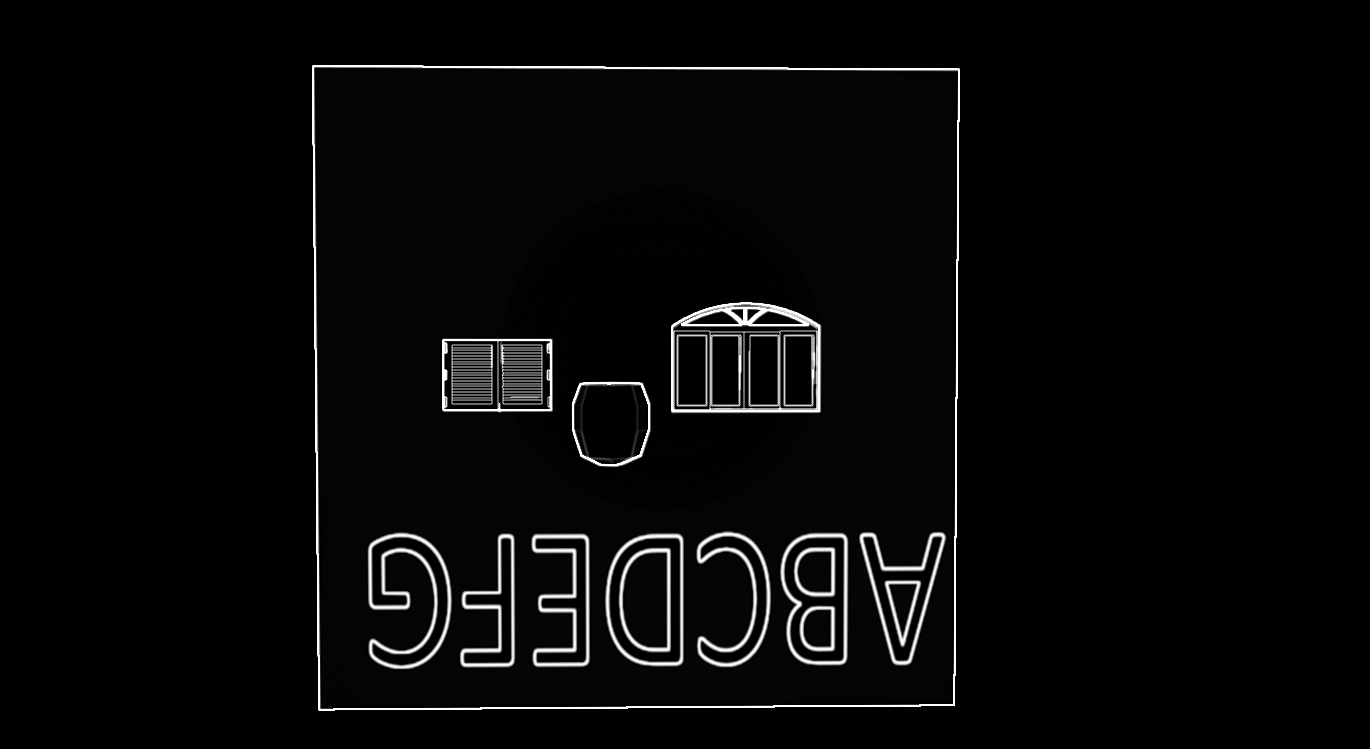
\includegraphics[scale=0.2]{images/aliased_value_example_3_temporal.png}
	\caption{Image made of the Aliased Values of each pixel.}\label{fig:aliasedval3}
\end{figure}

\subsection{Sharpen Filter Modifications}
With the current The Sharpen Filter, a color peak is created when the center pixel is bright and the neighboring pixels are dark, this is because dark colors are close to zero but the center pixel is still multiplied by $5$. An example of the worst possible case is having the center pixel as a bright color and the neighborhood’s pixels as pure black, which are represented as zero. Therefore, we normalized Sharpen Filter to avoid creating that color peak and to work better with bright pixels with dark neighborhoods. The Filter was changed from \ref{eq:sharpen} to:
\begin{equation} \label{eq:new_sharpen}
\centering
\begin{bmatrix*}[c]
0 & -0.25 &  0 \\
-0.25  &  2 & -0.25  \\
0 & -0.25  &  0
\end{bmatrix*}
\end{equation}

Equation \ref{eq:new_sharpen} shows the new Sharpen Filter Convolution Matrix used.


\chapter{Results}
In this chapter, we explain how we evaluated the improvements done to the Temporal Anti-Aliasing. We show the numerical and visual results obtained. Finally, we explain the results and their meaning compared to the previous implementation of TAA and other Anti-Aliasing solutions.
\section{Evaluation Methodology}
To evaluate the improvements achieved to the Temporal Anti-Aliasing technique we selected models and camera angles that place the technique under stress. Then, using the Testing Framework we developed, we proceed to render and save images of each of those models to compare how the technique behaves in comparison to the original TAA implementation and other Anti-Aliasing techniques to determine if the proposed techniques in this thesis provided images with better quality without incurring heavy memory usage or time consumption. Also, a special test was taken to measure if changing the Sharpen Filter was the sole mechanism providing an improvement.

The models used on the tests were:
\begin{itemize}
\item Pipe: A brown pipe with hard edges.
\item Window with Blinds: A blue window with closed blinds.
\item Arched Window: A blue window with an arch at the top.
\item Wall: A white wall with black text.
\item Sponza Atrium: exemplifies a general scene.
\item Sponza Atrium Flowers: exemplifies a cutout model.
\item Hairball: contains many fine details for its numerous fibers.
\end{itemize}

It is important to note that in Computer Graphics there are only common models used to test techniques, there is no standard per se. On this Master Thesis, we used two common models: the Sponza Atrium, which has many variations and it is commonly used to test many Computer Graphics techniques; and Hairball, which is sometimes used to test Ray and Path Tracing techniques. As well, an explanation why each model was selected is available under each test subsection.

Note that Sponza Atrium and Hairball models were downloaded from Morgan McGuire's Computer Graphics Archive \cite{McGuire2017Data}; the Pipe model is from Spencer Arts \cite{Spencer2010}; the Arched Window model is from Isabela H. \cite{Isabela2016}; and the Window with Blinds is from Channa Yim \cite{Channa2015}.

The tests were performed on the computer provided by Lund University which has the following specification:
\begin{itemize}
\setlength\itemsep{0em}
\item CPU: Intel(R) Core(TM) i7-3820 CPU @ 3.60GHz, 3601 Mhz, 4 Cores, 8 Logical Processors
\item RAM: 64.0 GB	
\item GPU: NVIDIA GeForce GTX 1080 with 8 GB of VRAM
\item Rendering Resolution when not zooming: 1600 x 900
\end{itemize}

\section{Results and Comparisons}
First, we need to know that the best possible value for MSE and RMSD is zero, meaning that there is no error; that having a high PSNR and SNR value means it is better because the noise, which is the denominator in the equation of this metric, is close to zero; and, finally, that having an SSIM of $1$ means that the image is structurally the same as the ground truth, while having a value of $0$ means that it is structurally different. For the SSIM maps, each pixel represents its SSIM value; having a white color means that is structurally the same while having a darker color means that there are structural differences.

\subsection{Sharpen Filter}
For this test, we rendered the Sponza Atrium Model and a Static Sphere Model to evaluate the effects of the Normalized Sharpen Filter to the general quality of the rendered image, especially, regarding the blurring normally caused by TAA. Everything was rendered using both implementations of TAA with and without the Normalized Sharpen Filter to see if this change was the only improvement that was increasing the quality of the rendered image. The scene was selected for the test because it provided an example of a general scene that should not generate any blur. As we see from the Table \ref{tab:sharpen_res}, even if the Master Thesis TAA and the Uncharted TAA used the new Sharpen Filter, our other improvements still rendered a higher quality image. If we zoom on Figure \ref{fig:sharpen_render} From Figure \ref{fig:sharpen_ssim} we can see that the Normalized Sharpen Filter contributes reducing the artifacts in the rendered image, as there are almost no dark areas on the SSIM maps of the TAA's using it.

% Table generated by Excel2LaTeX from sheet 'Sharpen Filter'
\begin{table}[!hbt]
	\small
	\centering
	\caption{Sharpen Filter Test numerical results}
	\begin{tabular}{|m{2.5em}|c|c|c|c|c|}
		\hline
		\multicolumn{6}{|c|}{\textbf{Sharpen Filter Test}} \\
		\hline
		\textbf{\makecell{\diagbox[height=3em,innerwidth=2.5em]{Tests}{AA}}} & \textbf{\makecell{Uncharted \\ TAA \\ Not \\ Normalized}} & \textbf{\makecell{Uncharted \\ TAA \\ Normalized}} & \textbf{\makecell{Master \\ TAA \\ Not \\ Normalized}} & \textbf{\makecell{Master \\ TAA \\ Normalized}} & \textbf{\makecell{Best} } \\
		\hline
		MSE   & 149.271 & 8.835 & 148.036 & 8.224 & \textbf{\makecell{\scriptsize Master \\ \scriptsize TAA \\ \scriptsize Normalized}} \\
		\hline
		RMSD  & 12.218 & 2.972 & 12.167 & 2.868 & \textbf{\makecell{\scriptsize Master \\ \scriptsize TAA \\ \scriptsize Normalized}} \\
		\hline
		Peak-SNR  & 26.391 & 38.669 & 26.427 & 38.980 & \textbf{\makecell{\scriptsize Master \\ \scriptsize TAA \\ \scriptsize Normalized}} \\
		\hline
		SNR   & 16.245 & 28.522 & 16.281 & 28.833 & \textbf{\makecell{\scriptsize Master \\ \scriptsize TAA \\ \scriptsize Normalized}} \\
		\hline
		SSIM  & 0.932 & 0.992 & 0.933 & 0.992 & \textbf{\makecell{\scriptsize Master \\ \scriptsize TAA \\ \scriptsize Normalized}} \\
		\hline
	\end{tabular}%
	\label{tab:sharpen_res}%
\end{table}%

\begin{figure}[H]
	\centering
	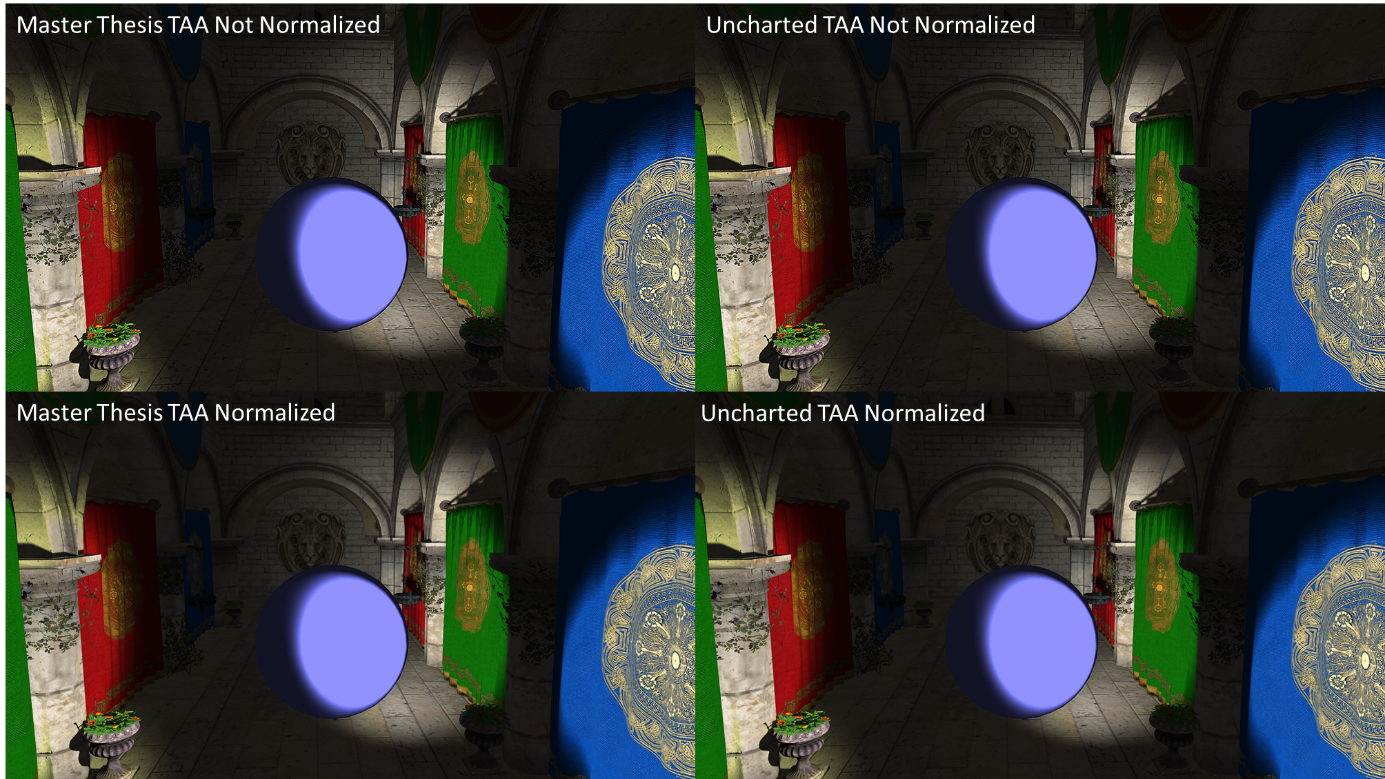
\includegraphics[scale=0.9]{images/results/sharpen_test_render.png}
	\caption{Rendered Images comparison.}\label{fig:sharpen_render}
\end{figure}

\begin{figure}[H]
	\centering
	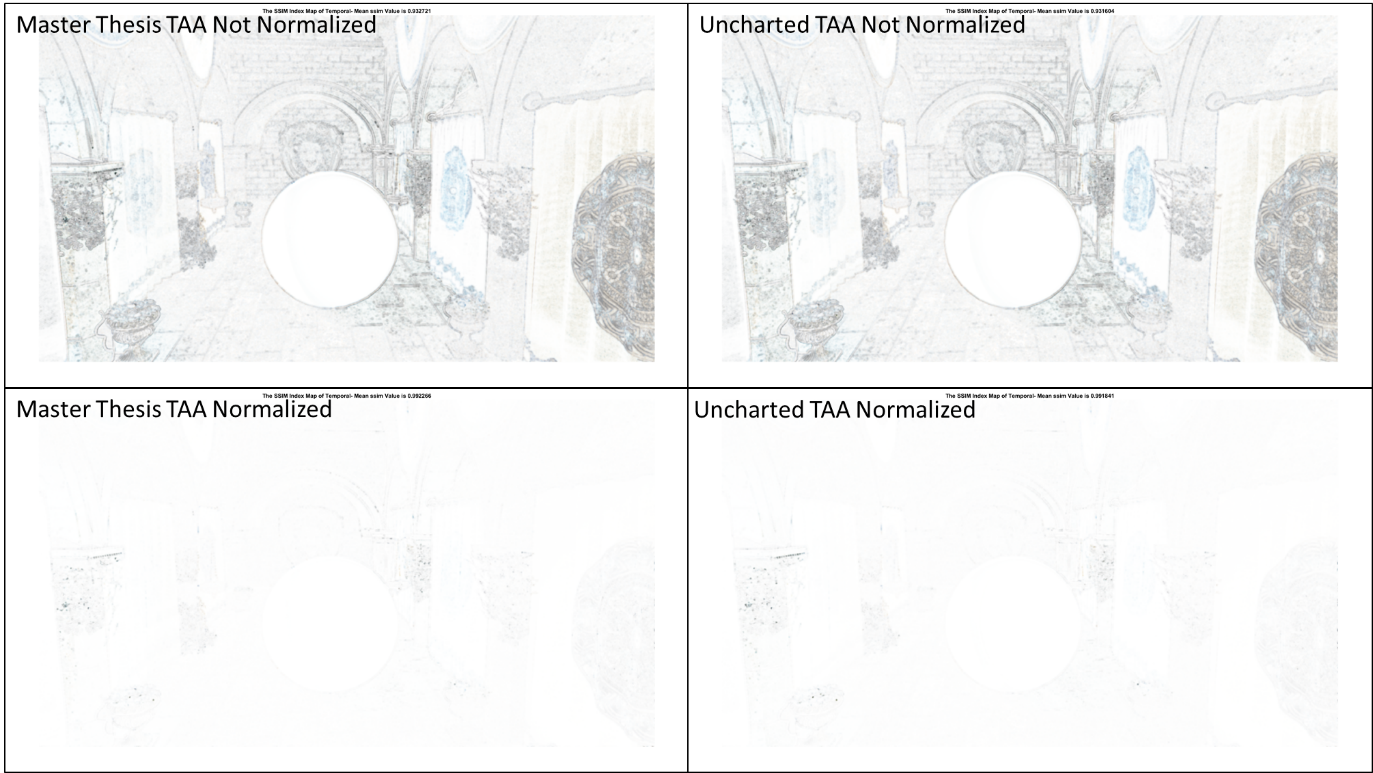
\includegraphics[scale=0.9]{images/results/sharpen_test_ssim.png}
	\caption{SSIM Maps comparison.}\label{fig:sharpen_ssim}
\end{figure}

\subsection{Pipe}
For this test, we rendered the Pipe Model in order to test how the improvements behaved when rendering a model with hard edges. We wanted to test if our improvements reduced the amount of blur around those hard edges while still fixing the aliasing problem. We rendered the Pipe twice, the first time using a regular camera angle, for normal aliasing around the edges, and a skewed camera angle, for increased aliasing effects. As we see from the results, TAA with our improvements is at the same quality level as SMAA. 

\subsubsection{Regular}
When we zoom and compare Figure \ref{fig:pipe_regular_truth} with the rendered images in Figure \ref{fig:pipe_regular_render}, especially around the edges, we observe that there is a reduction of blurring in the Master Thesis TAA in comparison with the Uncharted TAA. As well, we observe that the Uncharted TAA generates bright colors around the edges which should not be there; this is easier to observe as the dark edges on the SSIM map of the Uncharted TAA on Figure \ref{fig:pipe_regular_render}. Furthermore, Table \ref{tab:pipe_regular} confirm us that the Master Thesis TAA reaches almost the same quality as SMAA.

% Table generated by Excel2LaTeX from sheet 'Pipe Regular'
\begin{table}[!hbt]	
	\small
	\centering
	\caption{Numerical results of the Pipe Test with regular camera inclination.}
	\begin{tabular}{|l|c|c|c|c|c|c|c|}
		\hline
		\multicolumn{8}{|c|}{\textbf{Pipe Regular Test}} \\
		\hline
		\textbf{\diagbox{Tests}{AA}} & \textbf{No AA} & \textbf{FXAA}  & \textbf{SMAA}  & \textbf{\makecell{Uncharted \\ TAA}} & \textbf{\makecell{Master \\ TAA}} & \textbf{Best} & \textbf{\makecell{Master \\ TAA \\ Against \\ Best}} \\
		\hline
		MSE   & 8.608 & 3.573 & 1.278 & 14.602 & 1.574 & SMAA  & -0.296 \\
		\hline
		RMSD  & 2.934 & 1.890 & 1.130 & 3.821 & 1.254 & SMAA  & -0.124 \\
		\hline
		Peak-SNR  & 38.782 & 42.601 & 47.066 & 36.487 & 46.162 & SMAA  & 0.904 \\
		\hline
		SNR   & 36.451 & 40.270 & 44.735 & 34.156 & 43.831 & SMAA  & 0.904 \\
		\hline
		SSIM  & 0.999 & 0.999 & 1.000 & 0.996 & 1.000 & SMAA  & 0.000 \\
		\hline
	\end{tabular}%
	\label{tab:pipe_regular}%
\end{table}%

\begin{figure}[H]
	\centering
	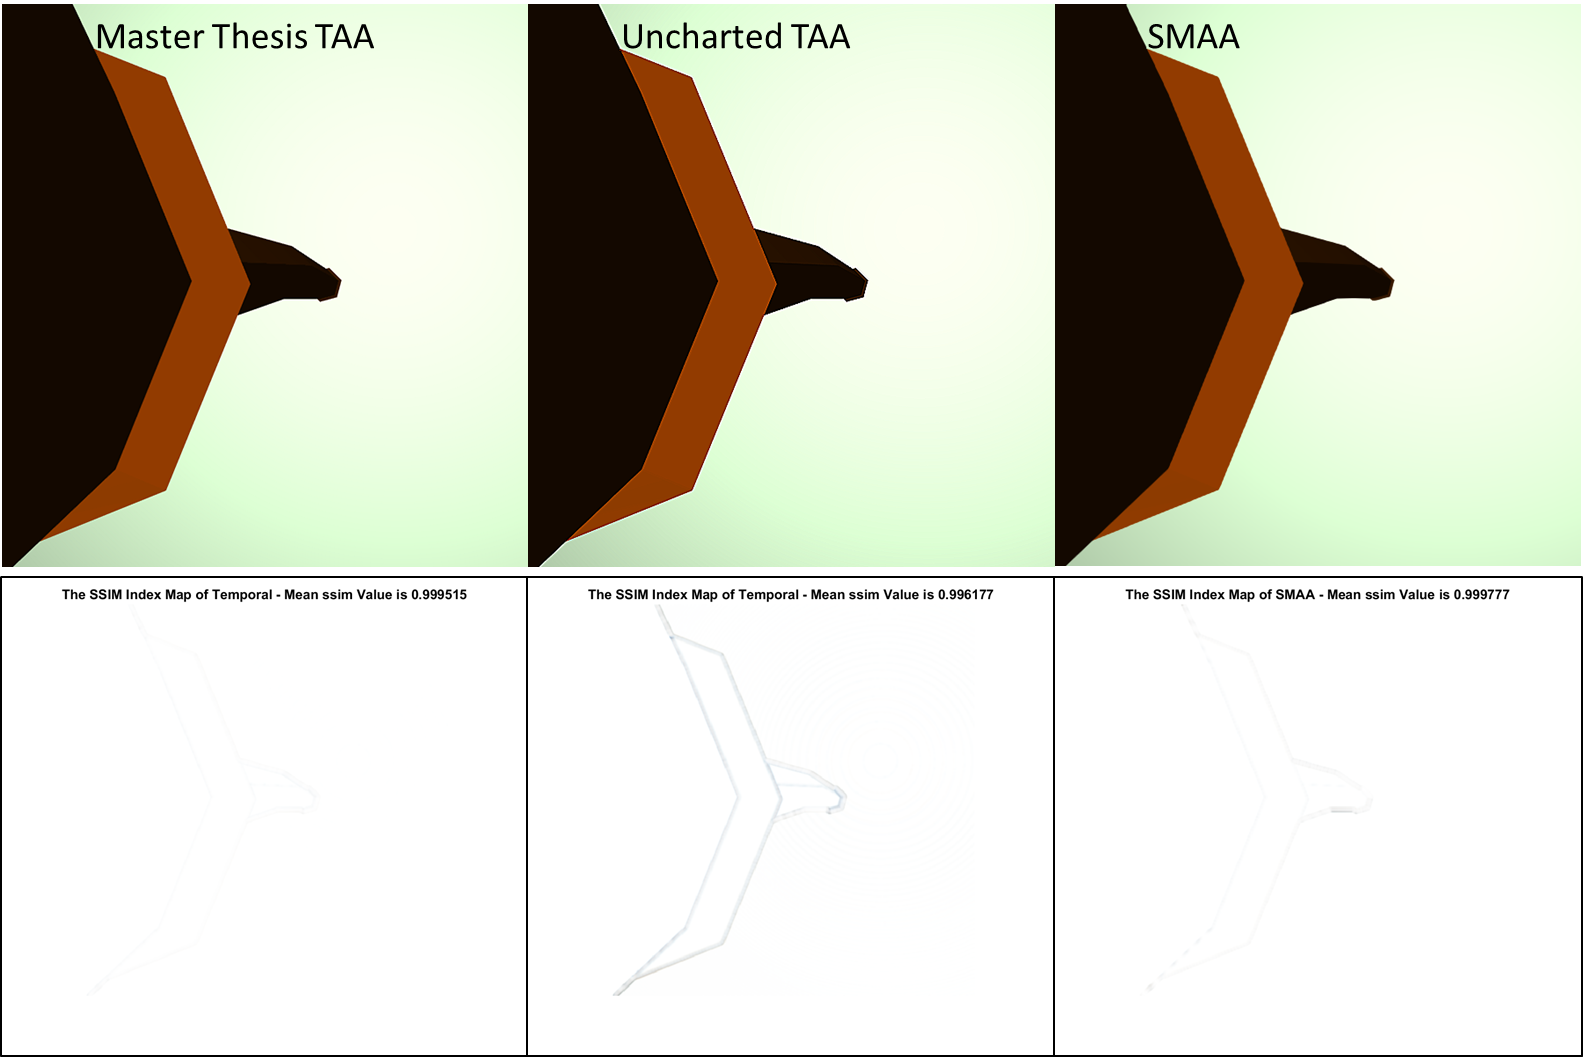
\includegraphics[scale=0.5]{images/results/pipe_regular.png}
	\caption{Pipe Regular comparison between Master Thesis TAA, Uncharted TAA, and SMAA.}\label{fig:pipe_regular_render}
\end{figure}

\begin{figure}[H]
	\centering
	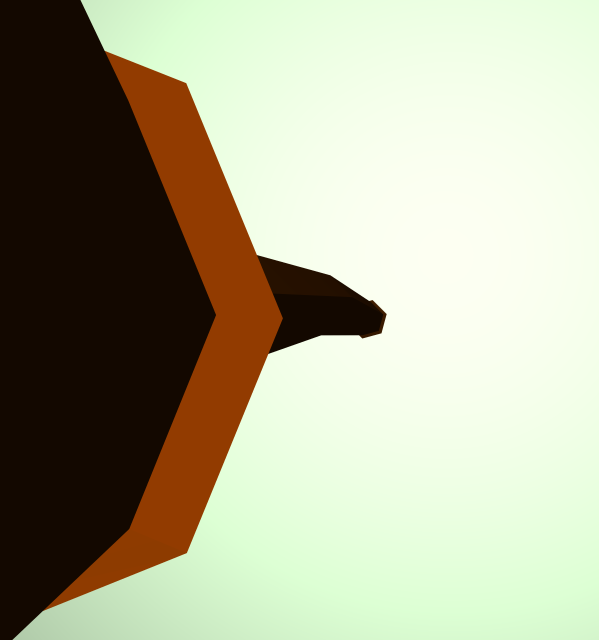
\includegraphics[scale=0.2]{images/results/pipe_regular_sobel_ground_truth.png}
	\caption{Pipe Regular Test ground truth.}\label{fig:pipe_regular_truth}
\end{figure}


\subsubsection{With Camera Inclination}
Zooming and comparing the Figures \ref{fig:pipe_inclination_render} and \ref{fig:pipe_inclination_truth}, we can observe that the Master TAA is the most similar to the Ground Truth. From the SSIM map of the Uncharted TAA, we notice that blurring is being generated around the edges. 

Finally, from Figure \ref{fig:pipe_inclination_render} and Table \ref{fig:pipe_inclination_truth} we note that SMAA is not properly detecting the upper edge of the pipe, when zoomed we observe a small staircase forming around the edge.  This is due to the fact that the camera was set up with a skewed inclination which pushed to the limit the edge detection techniques used in SMAA.

% Table generated by Excel2LaTeX from sheet 'Pipe with Inclination'
\begin{table}[H]
	\small
	\centering
	\caption{Numerical results of the Pipe Test with a skewed camera inclination.}
	\begin{tabular}{|l|c|c|c|c|c|c|c|}
		\hline
		\multicolumn{8}{|c|}{\textbf{Pipe with Camera Inclination Test}} \\
		\hline
		\textbf{\diagbox{Tests}{AA}} & \textbf{No AA} & \textbf{FXAA}  & \textbf{SMAA}  & \textbf{\makecell{Uncharted \\ TAA}} & \textbf{\makecell{Master \\ TAA}} & \textbf{Best} & \textbf{\makecell{Master \\ TAA \\ Against \\ Best}} \\
		\hline
		MSE   & 16.112 & 6.470 & 2.810 & 14.349 & 2.664 & Master TAA & 0.000 \\
		\hline
		RMSD  & 4.014 & 2.544 & 1.676 & 3.788 & 1.632 & Master TAA & 0.000 \\
		\hline
		Peak-SNR  & 36.059 & 40.022 & 43.644 & 36.563 & 43.876 & Master TAA & 0.000 \\
		\hline
		SNR   & 32.474 & 36.437 & 40.059 & 32.978 & 40.291 & Master TAA & 0.000 \\
		\hline
		SSIM  & 0.998 & 0.999 & 1.000 & 0.996 & 0.999 & SMAA  & 0.000 \\
		\hline
	\end{tabular}%
	\label{tab:pipe_inclination}%
\end{table}%

\begin{figure}[H]
	\centering
	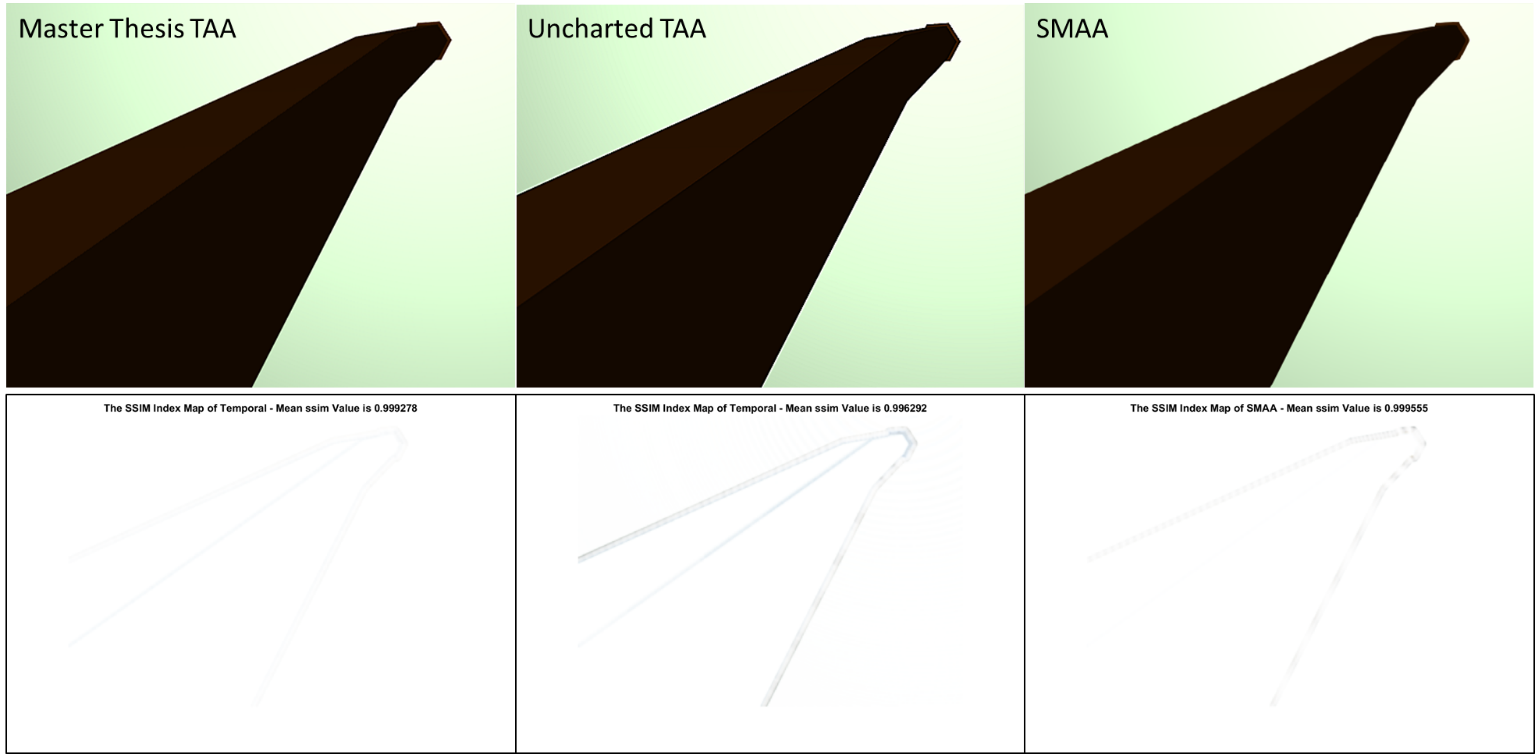
\includegraphics[scale=0.7]{images/results/pipe_inclination.png}
	\caption{Pipe with Camera Inclination comparison between Master Thesis TAA, Uncharted TAA, and SMAA.}\label{fig:pipe_inclination_render}
\end{figure}

\begin{figure}[H]
	\centering
	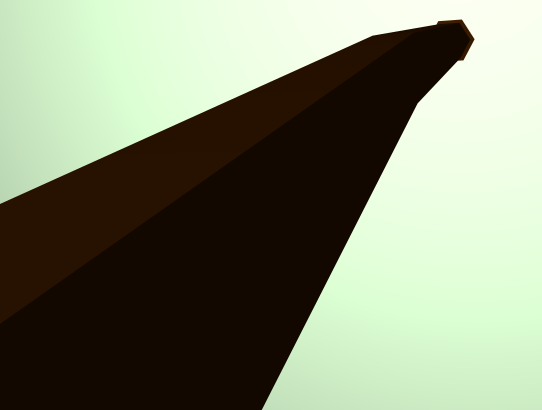
\includegraphics[scale=0.2]{images/results/pipe_with_inclination_sobel_ground_truth.png}
	\caption{Pipe with Camera Inclination Test ground truth.}\label{fig:pipe_inclination_truth}
\end{figure}


\subsection{Window with Blinds}
On this test, we used the Window with Blinds model for its small details at the blinds. We tested how our improvements behaved with this kind of details and discovered that it did not react in a proper way even if the numerical results showed otherwise.

From Figures \ref{fig:window_blind_render} and \ref{fig:window_blind_truth} we can observe it is complicated for the techniques to handle the small gaps between the blinds. From Figure \ref{fig:window_blind_render} and Table \ref{tab:window_blind}, we notice that the Master Thesis TAA and SMAA are able to reconstruct more details than the Uncharted TAA but, aesthetically and visually, we believe it is better the Uncharted TAA than the other techniques because those small gaps between the blinds flicker less when moving.

% Table generated by Excel2LaTeX from sheet 'Window Blind'
\begin{table}[H]
	\small
	\centering
	\caption{Numerical results of the Window with Blinds Test.}
	\begin{tabular}{|l|c|c|c|c|c|c|c|}
		\hline
		\multicolumn{8}{|c|}{\textbf{Window with Blinds Test}} \\
		\hline
		\textbf{\diagbox{Tests}{AA}} & \textbf{No AA} & \textbf{FXAA}  & \textbf{SMAA}  & \textbf{\makecell{Uncharted \\ TAA}} & \textbf{\makecell{Master \\ TAA}} & \textbf{Best} & \textbf{\makecell{Master \\ TAA \\ Against \\ Best}} \\
		\hline
		MSE   & 96.044 & 70.486 & 35.134 & 170.229 & 32.115 & Master TAA & 0.000 \\
		\hline
		RMSD  & 9.800 & 8.396 & 5.927 & 13.047 & 5.667 & Master TAA & 0.000 \\
		\hline
		Peak-SNR  & 28.306 & 29.650 & 32.674 & 25.820 & 33.064 & Master TAA & 0.000 \\
		\hline
		SNR   & 25.467 & 26.810 & 29.834 & 22.981 & 30.224 & Master TAA & 0.000 \\
		\hline
		SSIM  & 0.986 & 0.990 & 0.995 & 0.976 & 0.995 & Master TAA  & 0.000 \\
		\hline
	\end{tabular}%
	\label{tab:window_blind}%
\end{table}%

\begin{figure}[H]
	\centering
	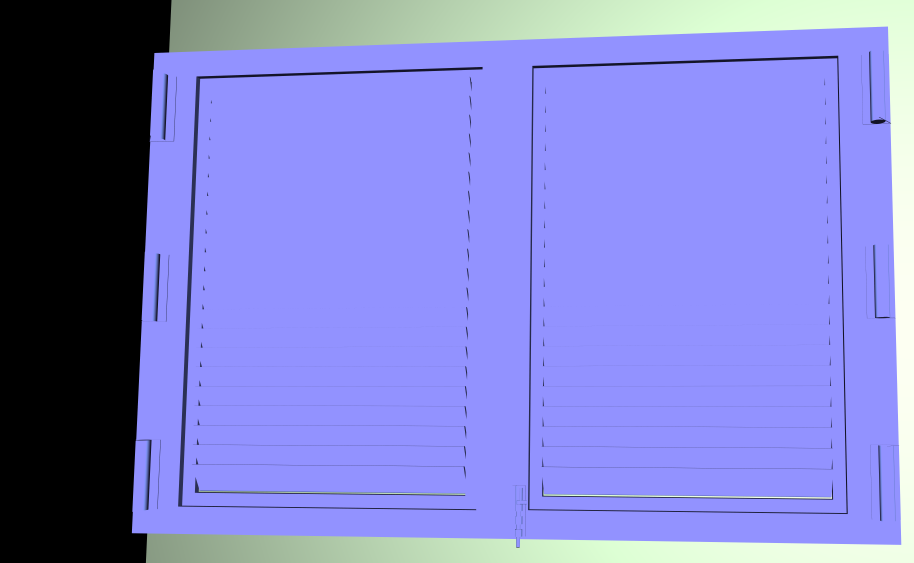
\includegraphics[scale=0.14]{images/results/window_blind_sobel_ground_truth.png}
	\caption{Window with Blinds ground truth.}\label{fig:window_blind_truth}
\end{figure}

\begin{figure}[H]
	\centering
	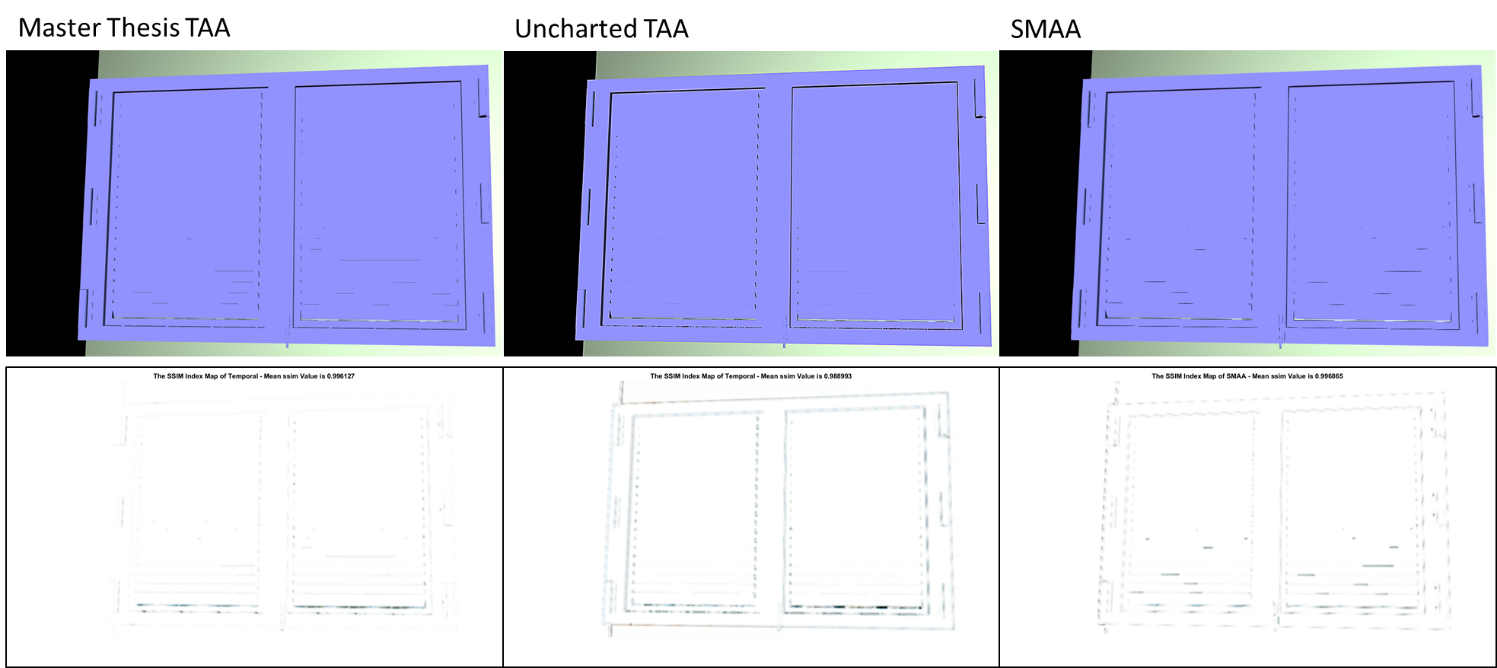
\includegraphics[scale=0.8]{images/results/window_blind.png}
	\caption{Window with Blinds comparison between Master Thesis TAA, Uncharted TAA, and SMAA.}\label{fig:window_blind_render}
\end{figure}



\subsection{Arched Window}
We used the Arched Window Model to test how our improved implementation with the small details of the window’s door and the aliasing from the arch. We can observe from Figures \ref{fig:window_arch_render} and \ref{fig:window_arch_truth} that for all the techniques, the small gaps around the window's door are hard to render. On some parts small gaps, we see that the techniques could not render it completely. Even though on Table \ref{tab:window_arch} SMAA appears to be the best, but we believe that the Uncharted TAA has the best visual quality because those incomplete gaps generate flickering when there is movement.
% Table generated by Excel2LaTeX from sheet 'Arched Window'
\begin{table}[H]
	\small
	\centering
	\caption{Numerical results of the Arched Window Test.}
	\begin{tabular}{|l|c|c|c|c|c|c|c|}
		\hline
		\multicolumn{8}{|c|}{\textbf{Arched Window Test}} \\
		\hline
		\textbf{\diagbox{Tests}{AA}} & \textbf{No AA} & \textbf{FXAA}  & \textbf{SMAA}  & \textbf{\makecell{Uncharted \\ TAA}} & \textbf{\makecell{Master \\ TAA}} & \textbf{Best} & \textbf{\makecell{Master \\ TAA \\ Against \\ Best}} \\
		\hline
		MSE   & 56.313 & 39.103 & 19.849 & 76.483 & 21.983 & SMAA  & -2.134 \\
		\hline
		RMSD  & 7.504 & 6.253 & 4.455 & 8.745 & 4.689 & SMAA  & -0.233 \\
		\hline
		Peak-SNR  & 30.625 & 32.209 & 35.153 & 29.295 & 34.710 & SMAA  & 0.443 \\
		\hline
		SNR   & 27.325 & 28.909 & 31.854 & 25.996 & 31.410 & SMAA  & 0.443 \\
		\hline
		SSIM  & 0.992 & 0.994 & 0.997 & 0.989 & 0.996 & SMAA  & 0.001 \\
		\hline
	\end{tabular}%
	\label{tab:window_arch}%
\end{table}%

\begin{figure}[H]
	\centering
	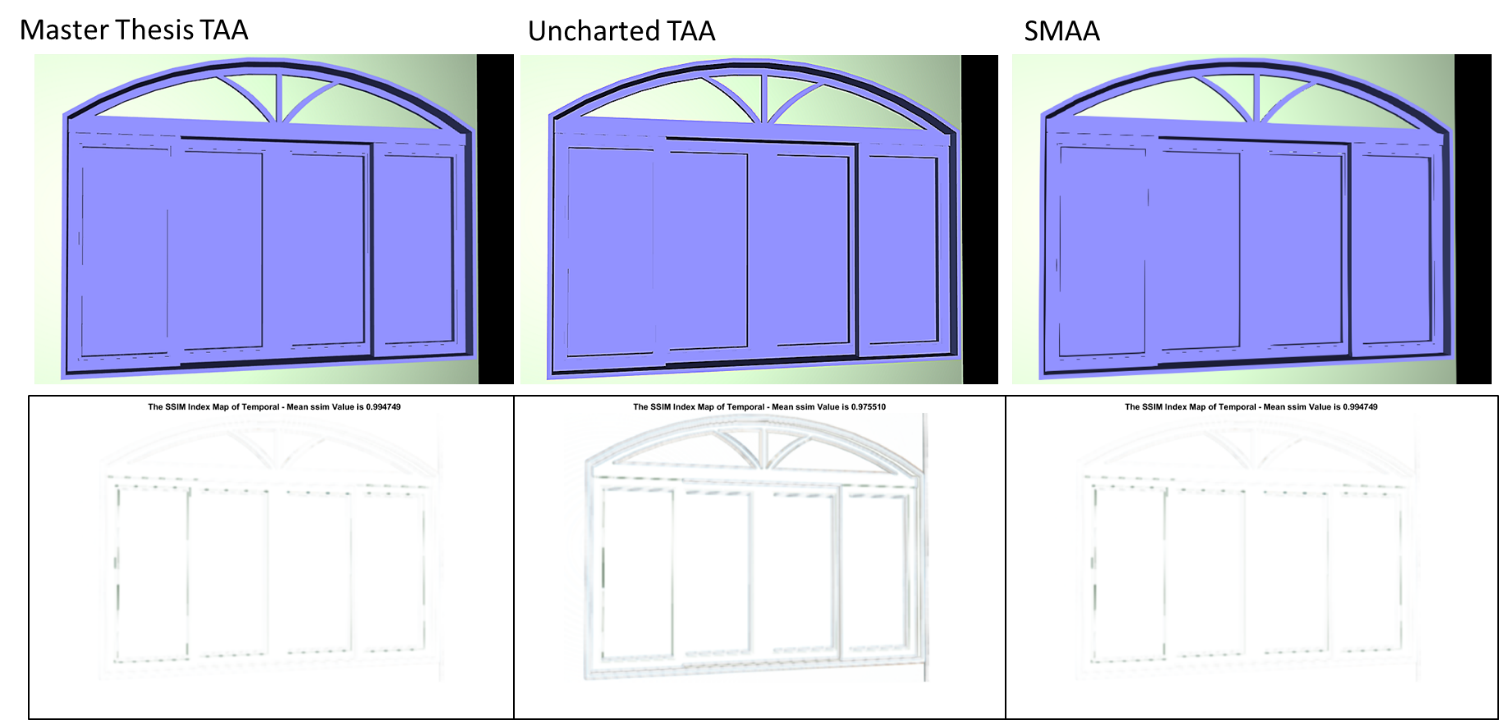
\includegraphics[scale=0.8]{images/results/window_arch.png}
	\caption{Arched Window comparison between Master Thesis TAA, Uncharted TAA, and SMAA.}\label{fig:window_arch_render}
\end{figure}

\begin{figure}[H]
	\centering
	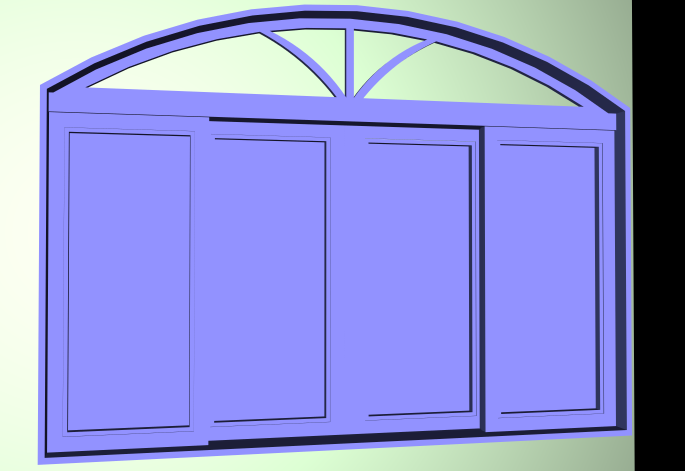
\includegraphics[scale=0.18]{images/results/window_arch_sobel_ground_truth.png}
	\caption{Arched Window ground truth.}\label{fig:window_arch_truth}
\end{figure}

\subsection{Sponza Atrium}
For this test, we wanted to analyze how the Master TAA implementation behaved with a general scene with lights and shadows, we used the Sponza Atrium Model with the Sphere Model being static in the center.

If we compare Figures \ref{fig:sponza_render} and \ref{fig:sponza_truth}, we can observe that the Uncharted TAA had blurring problems around all the edges, which is visible on its SSIM map; SMAA had problems with all the flowers, we can observe the flower shape on its SSIM map; and that the Master Thesis TAA only had minor problems with the flowers, as seen on the gray areas on its SSIM map. Furthermore, Table \ref{tab:sponza} confirm what we are observing on the visual results, as the Master Thesis TAA got the best scores on most of the test; the Uncharted TAA got the worst scores due to the edges problems; and SMAA got worse than normally scores due to the flowers problem.
% Table generated by Excel2LaTeX from sheet 'Sponza Table'
\begin{table}[H]
	\small
	\centering
	\caption{Numerical results of the Sponza Atrium Test.}
	\begin{tabular}{|l|c|c|c|c|c|c|c|}
		\hline
		\multicolumn{8}{|c|}{\textbf{Sponza Atrium Test}} \\
		\hline
		\textbf{\diagbox{Tests}{AA}} & \textbf{No AA} & \textbf{FXAA}  & \textbf{SMAA}  & \textbf{\makecell{Uncharted \\ TAA}} & \textbf{\makecell{Master \\ TAA}} & \textbf{Best} & \textbf{\makecell{Master \\ TAA \\ Against \\ Best}} \\
		\hline
		MSE   & 13.458 & 8.290 & 8.610 & 42.728 & 3.972 & Master TAA & 0.000 \\
		\hline
		RMSD  & 3.669 & 2.879 & 2.934 & 6.537 & 1.993 & Master TAA & 0.000 \\
		\hline
		Peak-SNR  & 36.841 & 38.945 & 38.781 & 31.824 & 42.141 & Master TAA & 0.000 \\
		\hline
		SNR   & 20.056 & 22.160 & 21.996 & 15.038 & 25.356 & Master TAA & 0.000 \\
		\hline
		SSIM  & 0.988 & 0.991 & 0.991 & 0.938 & 0.991 & Master TAA  & 0.000 \\
		\hline
	\end{tabular}%
	\label{tab:sponza}%
\end{table}%

\begin{figure}[H]
	\centering
	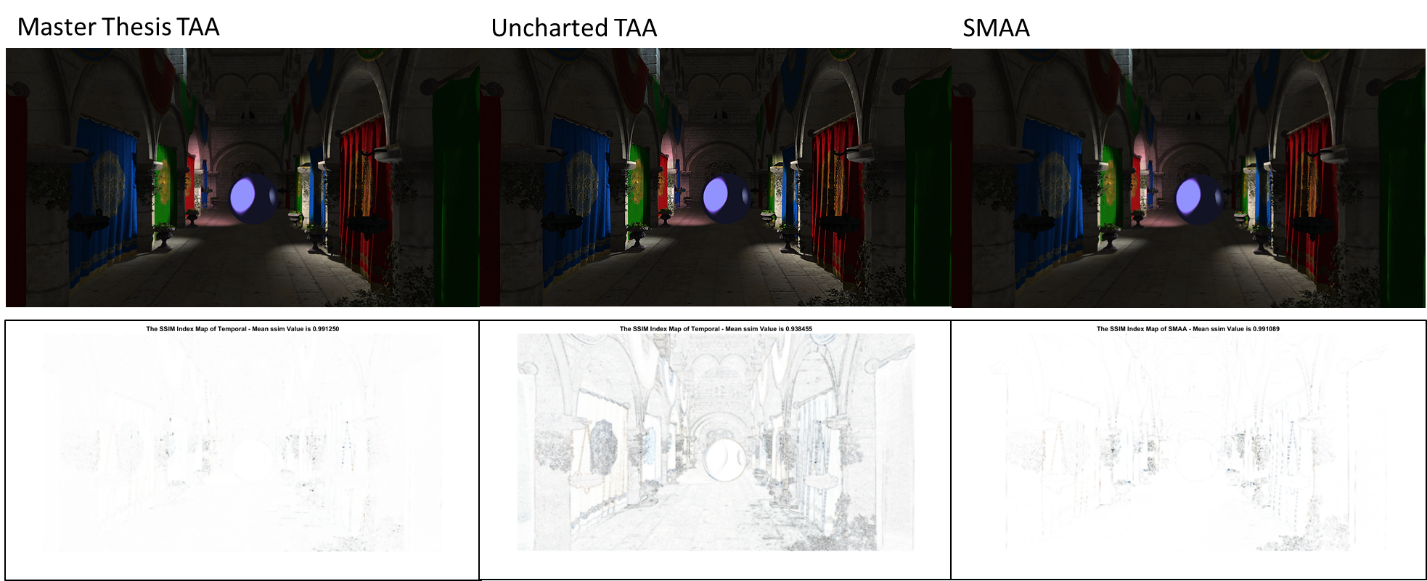
\includegraphics[scale=0.9]{images/results/sponza.png}
	\caption{Sponza Atrium comparison between Master Thesis TAA, Uncharted TAA, and SMAA.}\label{fig:sponza_render}
\end{figure}

\begin{figure}[H]
	\centering
	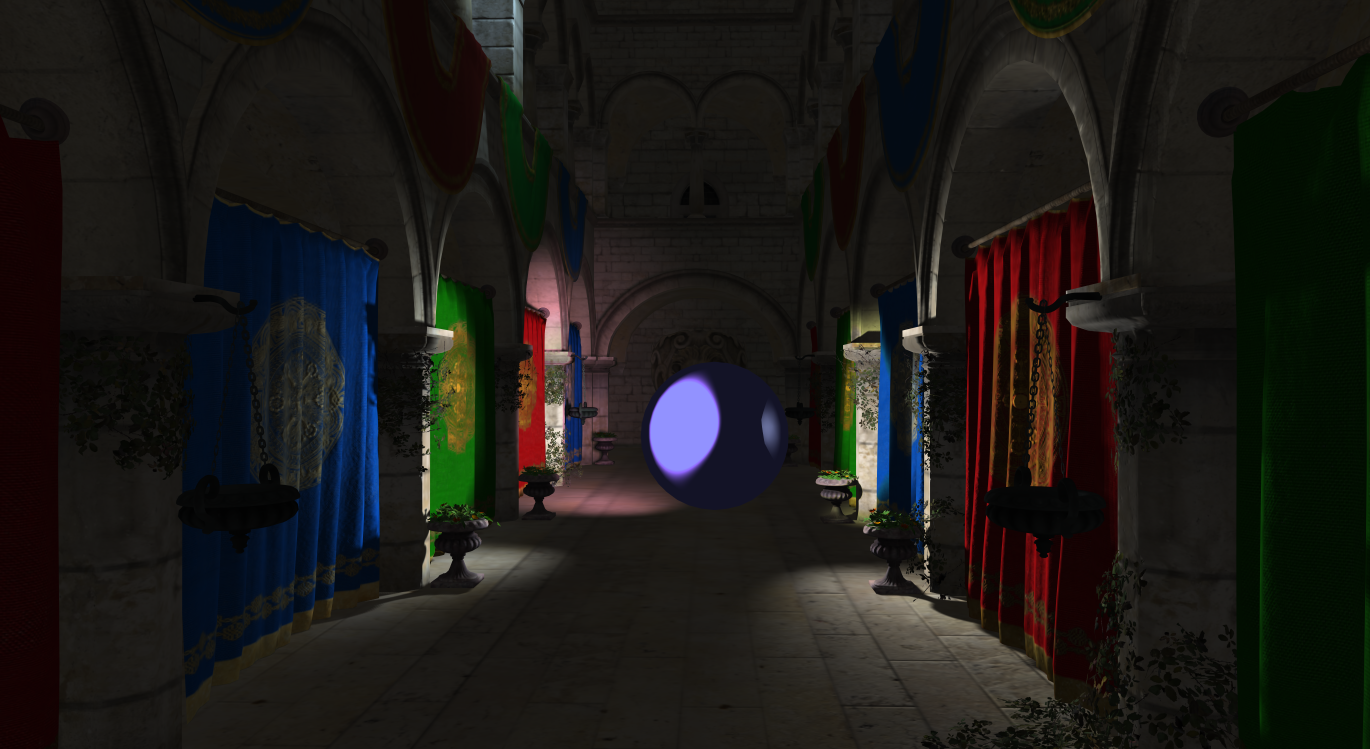
\includegraphics[scale=0.1]{images/results/sponza_sobel_ground_truth.png}
	\caption{Sponza Atrium ground truth.}\label{fig:sponza_truth}
\end{figure}

\subsection{Sponza Atrium Flowers}
On this test, we looked at how do our improvements handle the details of a model with transparent parts, as in the Flowers from the Sponza Atrium Model, because the aliasing they present is considered hard to properly detect and correct.

From Figures \ref{fig:sponza_flowers_render} and \ref{fig:sponza_flowers_truth}, we observe the Uncharted TAA has many problems handling this type of model, especially if we look at its SSIM map; we notice that SMAA could not correct all the aliasing artifacts from the edges of the flowers, we see the edges of the flowers appear on its SSIM map; and, finally, we observe that the Master Thesis TAA corrected the most aliasing artifacts, some are still left as seen on its SSIM map on the gray areas. Furthermore, Table \ref{tab:sponza_flowers} confirm what we observe visually, as the Master TAA got the best scores and SMAA scored worse than average.

% Table generated by Excel2LaTeX from sheet 'Sponza Flowers'
\begin{table}[H]
	\small
	\centering
	\caption{Numerical results of the Sponza Atrium Flowers Test.}
	\begin{tabular}{|l|c|c|c|c|c|c|c|}
		\hline
		\multicolumn{8}{|c|}{\textbf{Sponza Atrium Flowers Test}} \\
		\hline
		\textbf{\diagbox{Tests}{AA}} & \textbf{No AA} & \textbf{FXAA}  & \textbf{SMAA}  & \textbf{\makecell{Uncharted \\ TAA}} & \textbf{\makecell{Master \\ TAA}} & \textbf{Best} & \textbf{\makecell{Master \\ TAA \\ Against \\ Best}} \\
		\hline
		MSE   & 122.795 & 66.062 & 72.279 & 490.281 & 36.162 & Master TAA & 0.000 \\
		\hline
		RMSD  & 11.081 & 8.128 & 8.502 & 22.142 & 6.013 & Master TAA & 0.000 \\
		\hline
		Peak-SNR  & 27.239 & 29.931 & 29.541 & 21.226 & 32.548 & Master TAA & 0.000 \\
		\hline
		SNR   & 19.590 & 22.282 & 21.891 & 13.577 & 24.899 & Master TAA & 0.000 \\
		\hline
		SSIM  & 0.959 & 0.975 & 0.972 & 0.863 & 0.985 & Master TAA & 0.000 \\
		\hline
	\end{tabular}%
	\label{tab:sponza_flowers}%
\end{table}%

\begin{figure}[H]
	\centering
	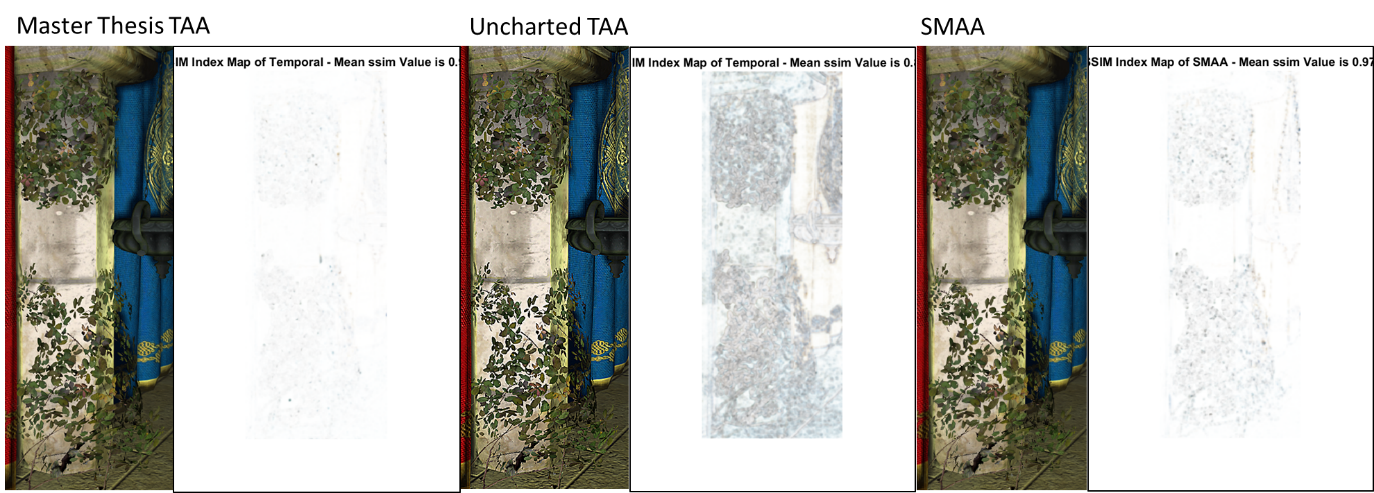
\includegraphics[scale=0.9]{images/results/sponza_flowers.png}
	\caption{Sponza Atrium Flowers comparison between Master Thesis TAA, Uncharted TAA, and SMAA.}\label{fig:sponza_flowers_render}
\end{figure}

\begin{figure}[H]
	\centering
	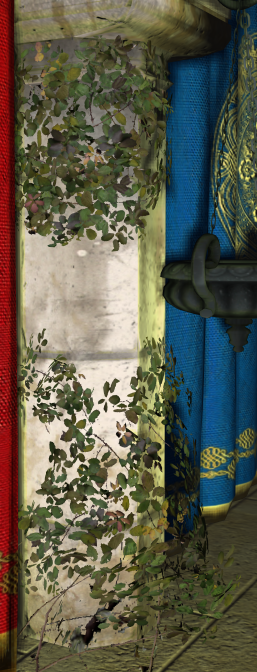
\includegraphics[scale=0.2]{images/results/sponza_flowers_sobel_ground_truth.png}
	\caption{Sponza Atrium Flowers ground truth.}\label{fig:sponza_flowers_truth}
\end{figure}

\subsection{Hard Edges}
For this test, we explored how the Master Thesis Implementation with many small details at a far distance and how it behaved with hard edges. We used both Windows Models for the small details and the Pipe and Wall Models for the hard edges. 

From Figures \ref{fig:hard_test_render} and \ref{fig:hard_test_truth}, we observe that the Master TAA is the best technique for handling all the edges from all the models, its SSIM map barely has any dark area and on Table \ref{tab:hard_test} it surpasses any other technique; the Uncharted TAA creates blurring around all the edges, this appears on its SSIM maps as all the edges are visible; and SMAA fail to correct some aliasing artifacts which we can observe on its SSIM map.

% Table generated by Excel2LaTeX from sheet 'Hard Test'
\begin{table}[H]
	\small
	\centering
	\caption{Numerical results of the Hard Edges Test.}
	\begin{tabular}{|l|c|c|c|c|c|c|c|}
		\hline
		\multicolumn{8}{|c|}{\textbf{Hard Edges Test}} \\
		\hline
		\textbf{\diagbox{Tests}{AA}} & \textbf{No AA} & \textbf{FXAA}  & \textbf{SMAA}  & \textbf{\makecell{Uncharted \\ TAA}} & \textbf{\makecell{Master \\ TAA}} & \textbf{Best} & \textbf{\makecell{Master \\ TAA \\ Against \\ Best}} \\
		\hline
		MSE   & 12.463 & 9.342 & 8.019 & 31.385 & 5.012 & Master TAA & 0.000 \\
		\hline
		RMSD  & 3.530 & 3.057 & 2.832 & 5.602 & 2.239 & Master TAA & 0.000 \\
		\hline
		Peak-SNR  & 37.174 & 38.426 & 39.090 & 33.164 & 41.131 & Master TAA & 0.000 \\
		\hline
		SNR   & 30.327 & 31.579 & 32.242 & 26.316 & 34.283 & Master TAA & 0.000 \\
		\hline
		SSIM  & 0.997 & 0.997 & 0.998 & 0.989 & 0.998 & Master TAA & 0.000 \\
		\hline
	\end{tabular}%
	\label{tab:hard_test}%
\end{table}%


\begin{figure}[H]
	\centering
	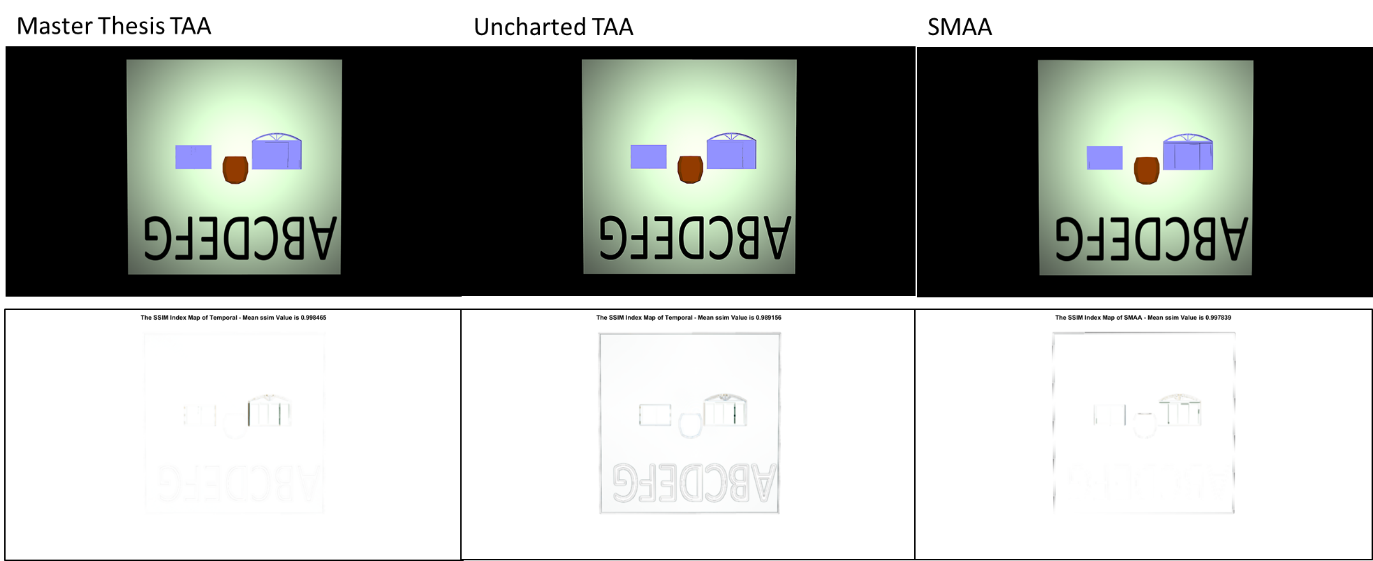
\includegraphics[scale=0.9]{images/results/hard_test.png}
	\caption{Hard Edges comparison between Master Thesis TAA, Uncharted TAA, and SMAA.}\label{fig:hard_test_render}
\end{figure}

\begin{figure}[H]
	\centering
	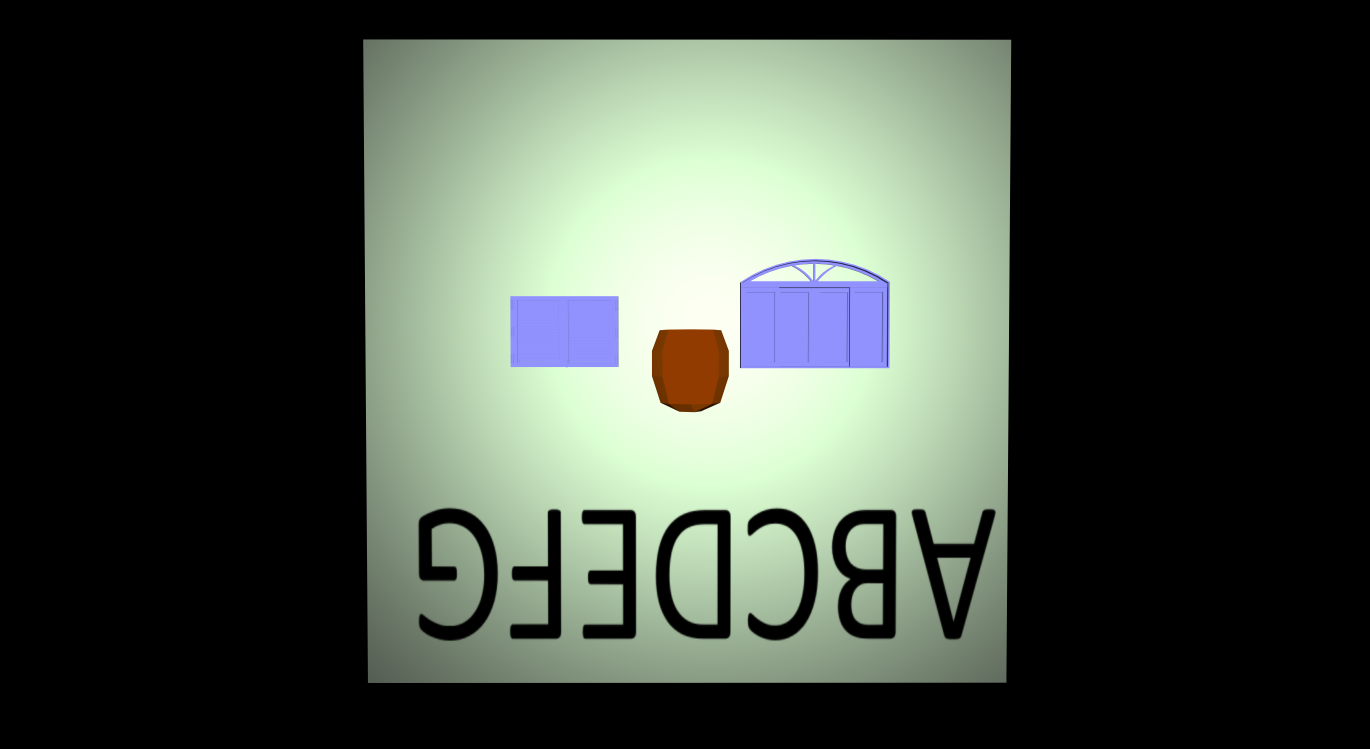
\includegraphics[scale=0.09]{images/results/hard_test_sobel_ground_truth.png}
	\caption{Hard Edges ground truth.}\label{fig:hard_test_truth}
\end{figure}


\subsection{Sphere Ghosting}
For this test, we wanted to measure how the improvements we performed decreased the effects of ghosting that were present in the Uncharted Implementation. For this reason, we selected the Sphere Model to move in the hall of the Sponza Atrium and rendered it under a camera angle that showed us ghosting trails. 

As we see from the visual results on Figure \ref{fig:sphere_ghosting}, ghosting effects were diminished in our implementation as the stripes visible on the Uncharted TAA are almost invisible on the Master Thesis TAA. Furthermore, in Table \ref{tab:sphere_ghosting} the average results on the Master TAA image metrics are better than the average from the Uncharted TAA. 

It is important to note that some metrics got an infinite result as they were exactly the same as the ground truth. This happens on some images in which the spheres cover the whole frame with a dark blue color. As well, the Test Index marks which test the associated result belongs to; on the averages we use Not Applicable (N\\A) because those results come from the average of all the tests. 
% Table generated by Excel2LaTeX from sheet 'Sphere Ghosting'
\begin{table}[H]
	\small
	\centering
	\caption{Numerical results summary of the 100 tests performed for the Sphere Ghosting Test.}
	\begin{tabular}{|l|c|c|c|c|}
		\hline
		\multicolumn{5}{|c|}{\textbf{Sphere Ghosting Test Summary}} \\
		\hline
		\multicolumn{1}{|c|}{\textbf{\diagbox{Tests}{AA}}} & \textbf{Uncharted TAA} & \textbf{Test Index} & \textbf{Master TAA} & \textbf{Test Index} \\
		\hline
		Best MSE & 0.000 & 63 & 0.000 & 63 \\
		\hline
		Worst MSE & 100.871 & 19 & 91.766 & 29 \\
		\hline
		Average MSE & 28.634 & N/A   & 19.501 & N/A \\
		\hline
		Best Peak-SNR & Inf   & 63 & Inf   & 63 \\
		\hline
		Worst Peak-SNR & 28.093 & 19 & 28.504 & 29 \\
		\hline
		Average Peak-SNR  & Inf   & N/A   & Inf   & N/A \\
		\hline
		Best SNR & Inf   & 63 & Inf   & 63 \\
		\hline
		Worst SNR & 16.818 & 11 & 18.524 & 29 \\
		\hline
		Average SNR  & Inf   & N/A   & Inf   & N/A \\
		\hline
		Best SSIM & 1.000 & 63 & 1.000 & 63 \\
		\hline
		Worst SSIM & 0.964 & 99 & 0.972 & 29 \\
		\hline
		Average SSIM & 0.965 & N/A   & 0.990 & N/A \\
		\hline
	\end{tabular}%
	\label{tab:sphere_ghosting}%
\end{table}%

\begin{figure}[H]
	\centering
	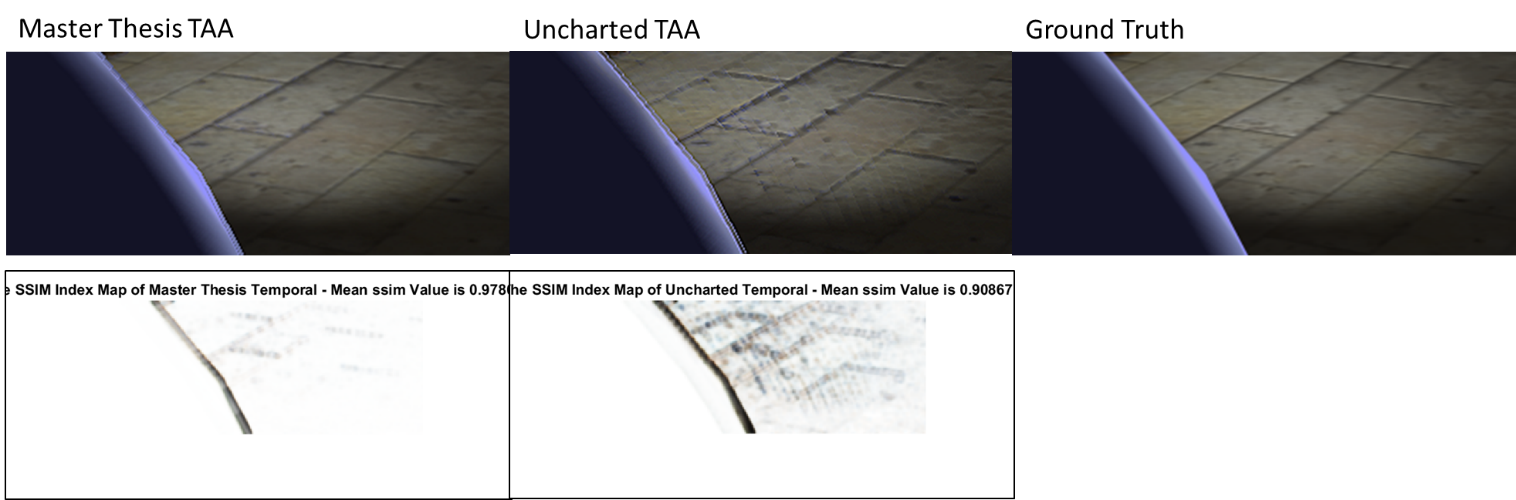
\includegraphics[scale=0.8]{images/results/sphere_ghosting.png}
	\caption{Example of Ghosting. Comparison between Master Thesis TAA, Uncharted TAA and Ground Truth on Test Number 19.}\label{fig:sphere_ghosting}
\end{figure}

\subsection{Hairball}
These tests were the hardest for all the techniques we tried. The Hairball Model contains many fibers with many details that provide a complex test for any Anti-Aliasing solution. We performed all the tests without light, to see the silhouette, and with light, to see how its reaction to the fibers affected all the Anti-Aliasing solutions. We did two sets of tests, the first one was static, to show us the behavior of blurring and aliasing correction; and the second set was rotating, to show us how ghosting behaved on the fibers. The results from the static tests were surprising, as we did not expect the Master Thesis Implementation to be the best handling the fibers because of the results in both windows tests.
\subsubsection{Static Shadow}
From Figures \ref{fig:hairball_static_shadow_render} and \ref{fig:hairball_static_shadow_truth}, we can observe that the Uncharted TAA has problems on most of the fibers, on its SSIM map this is visible as the big dark edge around Hairball; SMAA fails to correct aliasing on the smaller fibers, we observe this as the gray areas around the Hairball model on the SSIM map; and, finally, we notice that the Master TAA is the best at handling the fibers, they look smooth as in the original model, and its SSIM map has the least amount of dark areas. Also, from Table \ref{tab:hairball_static_shadow} we can confirm that the Master TAA is the best at rendering the static shadow Hairball by a relatively big margin compared to the other techniques.

% Table generated by Excel2LaTeX from sheet 'Hairball Static Shadow'
\begin{table}[!hbt]
	\small
	\centering
	\caption{Numerical results of the Hairball Static Shadow Test.}
	\begin{tabular}{|l|c|c|c|c|c|c|c|}
		\hline
		\multicolumn{8}{|c|}{\textbf{Hairball Static Shadow Test}} \\
		\hline
		\textbf{\diagbox{Tests}{AA}} & \textbf{No AA} & \textbf{FXAA}  & \textbf{SMAA}  & \textbf{\makecell{Uncharted \\ TAA}} & \textbf{\makecell{Master \\ TAA}} & \textbf{Best} & \textbf{\makecell{Master \\ TAA \\ Against \\ Best}} \\
		\hline
		MSE   & 44.367 & 21.101 & 25.379 & 88.976 & 10.293 & Master TAA & 0.000 \\
		\hline
		RMSD  & 6.661 & 4.594 & 5.038 & 9.433 & 3.208 & Master TAA & 0.000 \\
		\hline
		Peak-SNR  & 31.660 & 34.888 & 34.086 & 28.638 & 38.005 & Master TAA & 0.000 \\
		\hline
		SNR   & 18.808 & 22.036 & 21.234 & 15.786 & 25.154 & Master TAA & 0.000 \\
		\hline
		SSIM  & 0.962 & 0.978 & 0.974 & 0.934 & 0.985 & Master TAA & 0.000 \\
		\hline
	\end{tabular}%
	\label{tab:hairball_static_shadow}%
\end{table}%

\begin{figure}[H]
	\centering
	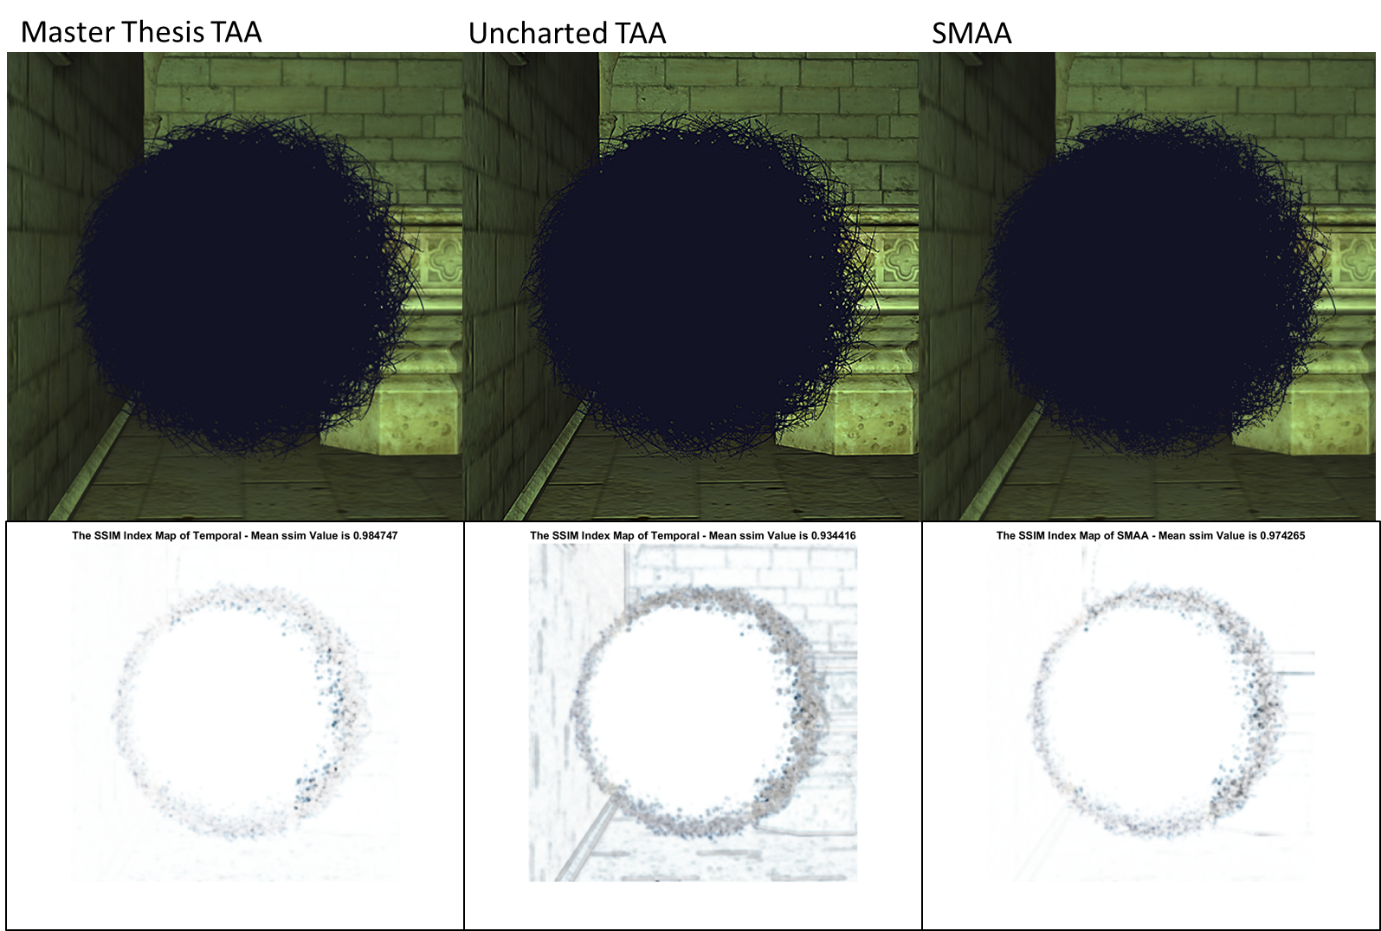
\includegraphics[scale=0.9]{images/results/hairball_static_shadow.png}
	\caption{Hairball Static Shadow comparison between Master Thesis TAA, Uncharted TAA, and SMAA.}\label{fig:hairball_static_shadow_render}
\end{figure}

\begin{figure}[H]
	\centering
	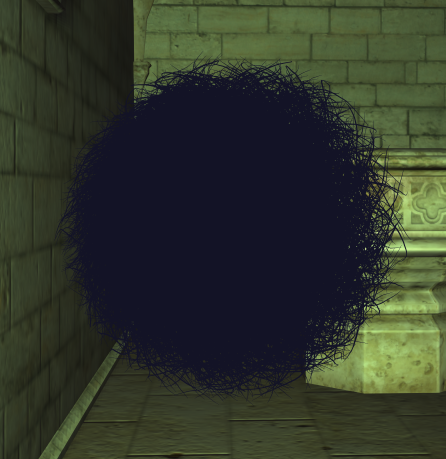
\includegraphics[scale=0.3]{images/results/hairball_sobel_ground_truth.png}
	\caption{Hairball Static Shadow ground truth.}\label{fig:hairball_static_shadow_truth}
\end{figure}


\subsubsection{Static Light}
From Figures \ref{tab:hairball_static_lighted} and \ref{fig:hairball_static_lighted_truth}, we observe that the Uncharted TAA generated wrong bright colors around all the fibers, on its SSIM this appears as the complete model is dark; SMAA fails to correct a high amount of fibers, they appear aliased on the rendered image and its SSIM map contains many dark zones; and, finally, we can observe that the Master TAA has the smoothest edges of all the rendered images, on its SSIM map and on Table \ref{tab:hairball_static_lighted} we notice that there still errors but they are smaller by a large margin compared to any other technique.

% Table generated by Excel2LaTeX from sheet 'Hairball Static Lighted'
\begin{table}[H]
	\small
	\centering
	\caption{Numerical results of the Hairball Static Light Test.}
	\begin{tabular}{|l|c|c|c|c|c|c|c|}
		\hline
		\multicolumn{8}{|c|}{\textbf{Hairball Static Light Test}} \\
		\hline
		\textbf{\diagbox{Tests}{AA}} & \textbf{No AA} & \textbf{FXAA}  & \textbf{SMAA}  & \textbf{\makecell{Uncharted \\ TAA}} & \textbf{\makecell{Master \\ TAA}} & \textbf{Best} & \textbf{\makecell{Master \\ TAA \\ Against \\ Best}} \\
		\hline
		MSE   & 1294.649 & 649.940 & 847.702 & 1444.095 & 226.567 & Master TAA & 0.000 \\
		\hline
		RMSD  & 35.981 & 25.494 & 29.115 & 38.001 & 15.052 & Master TAA & 0.000 \\
		\hline
		Peak-SNR  & 17.009 & 20.002 & 18.848 & 16.535 & 24.579 & Master TAA & 0.000 \\
		\hline
		SNR   & 8.446 & 11.439 & 10.285 & 7.971 & 16.015 & Master TAA & 0.000 \\
		\hline
		SSIM  & 0.801 & 0.865 & 0.841 & 0.785 & 0.937 & Master TAA & 0.000 \\
		\hline
	\end{tabular}%
	\label{tab:hairball_static_lighted}%
\end{table}%

\begin{figure}[H]
	\centering
	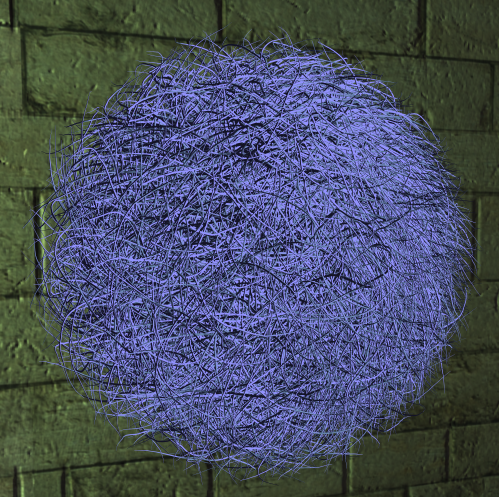
\includegraphics[scale=0.2]{images/results/hairball_light_sobel_ground_truth.png}
	\caption{Hairball Static Lighted ground truth.}\label{fig:hairball_static_lighted_truth}
\end{figure}

\begin{figure}[H]
	\centering
	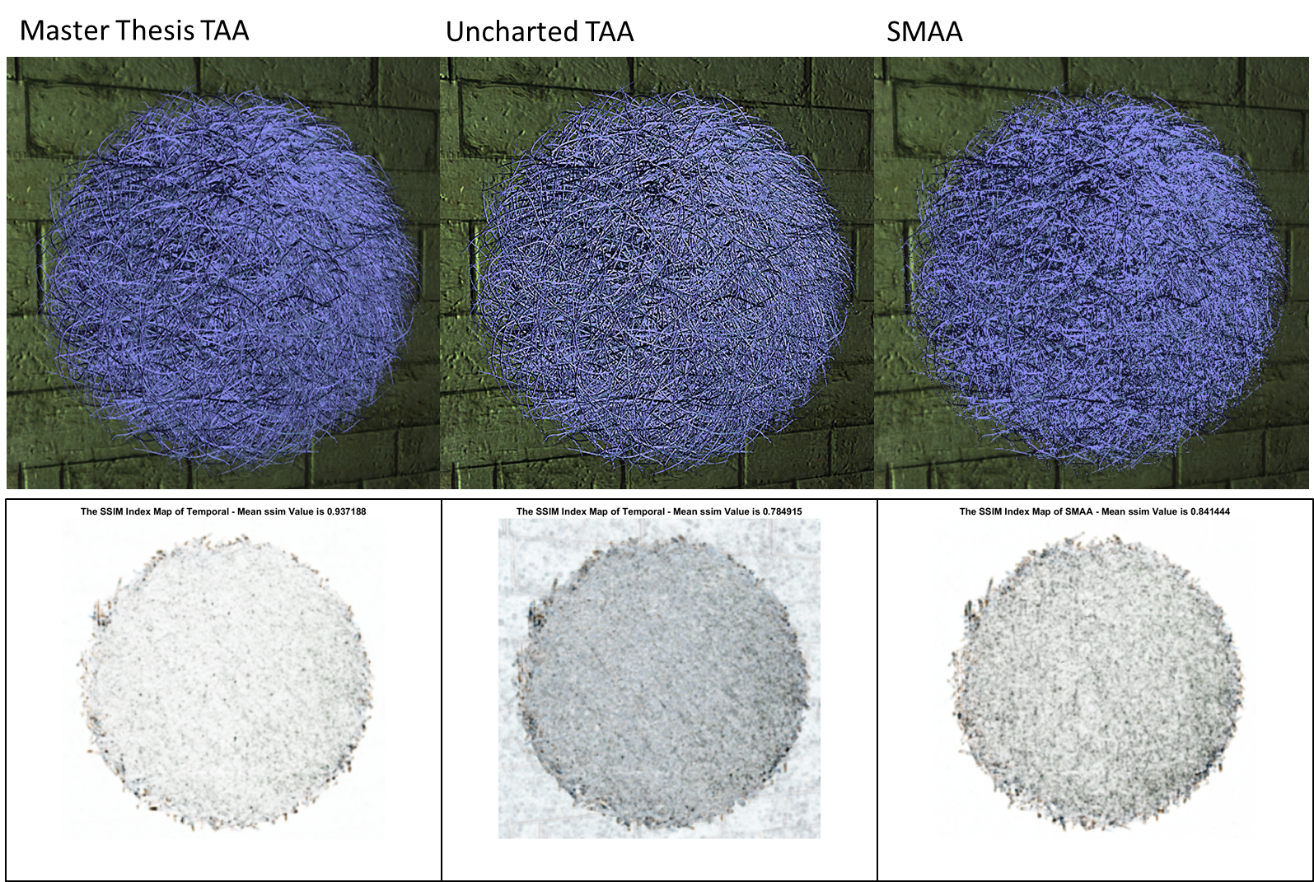
\includegraphics[scale=0.9]{images/results/hairball_static_lighted.png}
	\caption{Hairball Static Lighted comparison between Master Thesis TAA, Uncharted TAA, and SMAA.}\label{fig:hairball_static_lighted_render}
\end{figure}


\subsubsection{Ghosting Shadow}
From Figure \ref{fig:hairball_ghosting_shadow}, we can observe that both implementations generate blurriness around the fibers edges, this is visible on both SSIM maps as the dark ring around the model. On Table \ref{tab:hairball_ghosting_shadow} we observe that the Master Thesis TAA is numerically better than the Uncharted TAA. As well, the Test Index on Table \ref{tab:hairball_ghosting_shadow} marks which test the associated result belongs to; on the averages we use Not Applicable (N\\A) because those results come from the average of all the tests. 

% Table generated by Excel2LaTeX from sheet 'Hairball Ghosting Shadow'
\begin{table}[H]
	\small
	\centering
	\caption{Numerical results summary of the 100 tests performed for the Hairball Ghosting Shadow Test.}
	\begin{tabular}{|l|c|c|c|c|}
		\hline
		\multicolumn{5}{|c|}{\textbf{Hairball Ghosting Shadow Test Summary}} \\
		\hline
		\multicolumn{1}{|c|}{\textbf{\diagbox{Tests}{AA}}} & \textbf{Uncharted TAA} & \textbf{Test Index} & \textbf{Master TAA} & \textbf{Test Index} \\
		\hline
	    Best MSE & 70.261 & 17    & 32.692 & 0 \\
		\hline
		Worst MSE & 93.024 & 90    & 42.962 & 90 \\
		\hline
		Average MSE & 81.887 & N/A   & 38.534 & N/A \\
		\hline
		Best Peak-SNR & 29.664 & 17    & 32.986 & 0 \\
		\hline
		Worst Peak-SNR & 28.445 & 90    & 31.800 & 90 \\
		\hline
		Average Peak-SNR  & 29.009 & N/A   & 32.278 & N/A \\
		\hline
		Best SNR & 16.940 & 17    & 20.278 & 0 \\
		\hline
		Worst SNR & 15.846 & 90    & 19.201 & 90 \\
		\hline
		Average SNR  & 16.333 & N/A   & 19.602 & N/A \\
		\hline
		Best SSIM & 0.925 & 17    & 0.947 & 17 \\
		\hline
		Worst SSIM & 0.911 & 99    & 0.934 & 68 \\
		\hline
		Average SSIM & 0.913 & N/A   & 0.940 & N/A \\
		\hline
	\end{tabular}%
	\label{tab:hairball_ghosting_shadow}%
\end{table}%

\begin{figure}[H]
	\centering
	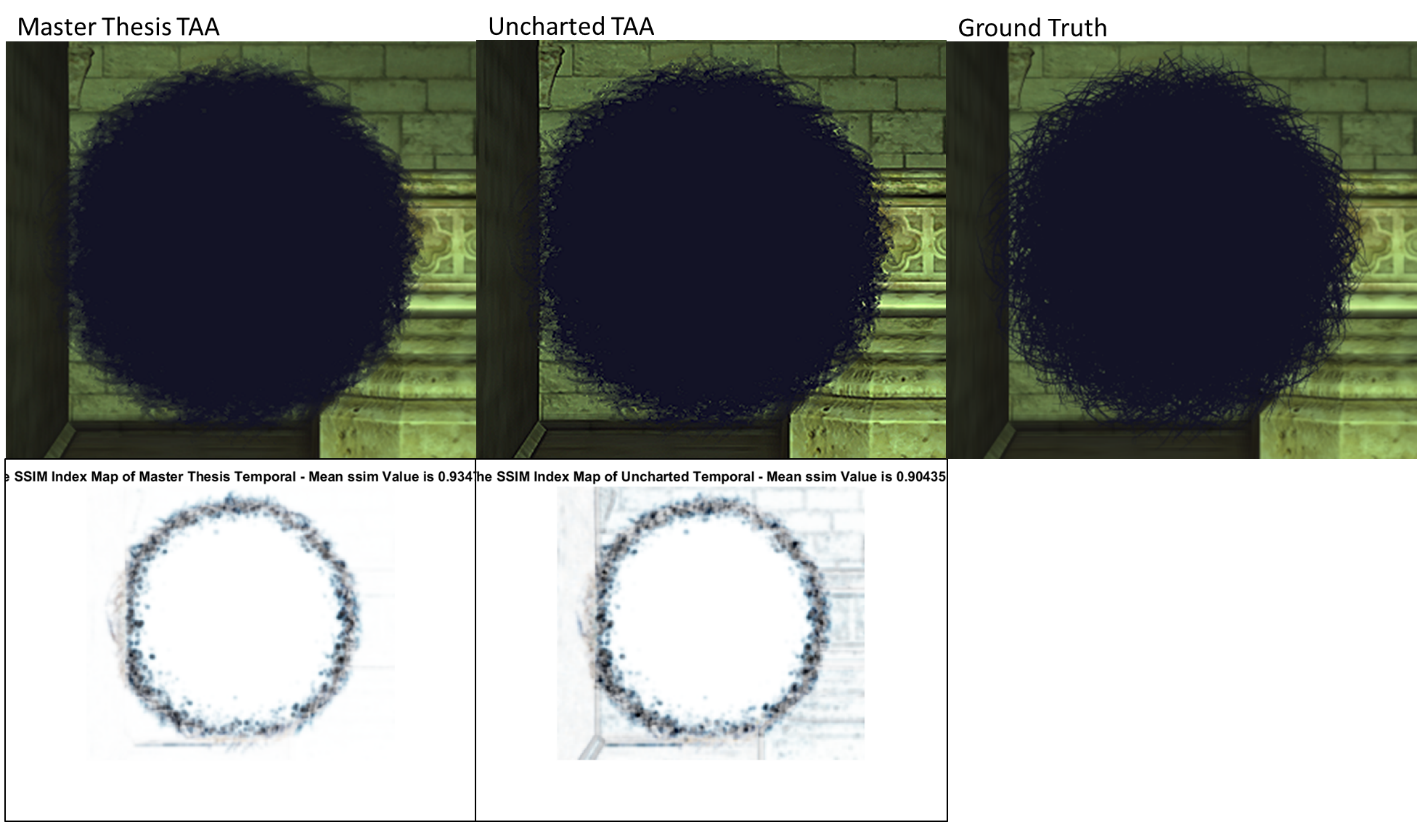
\includegraphics[scale=0.8]{images/results/hairball_ghosting_shadow.png}
	\caption{Ghosting comparison between Master Thesis TAA, Uncharted TAA and Ground Truth on Test Number 90.}\label{fig:hairball_ghosting_shadow}
\end{figure}

\subsubsection{Ghosting Light}
From Figure \ref{fig:hairball_ghosting_lighted} and Table \ref{tab:hairball_ghosting_lighted}, we observe that both techniques generate a high amount of blurring around the fibers. On both SSIM maps the blurring is visible as Hairball is seen as a big dark area. As well, the Test Index on Table \ref{tab:hairball_ghosting_lighted} marks which test the associated result belongs to; on the averages we use Not Applicable (N\\A) because those results come from the average of all the tests. 
% Table generated by Excel2LaTeX from sheet 'Hairball Ghosting Lighted'
\begin{table}[H]
	\small
	\centering
	\caption{Numerical results summary of the 100 tests performed for the Hairball Ghosting Light Test.}
	\begin{tabular}{|l|c|c|c|c|}
		\hline
		\multicolumn{5}{|c|}{\textbf{Hairball Light Shadow Test Summary}} \\
		\hline
		\multicolumn{1}{|c|}{\textbf{\diagbox{Tests}{AA}}} & \textbf{Uncharted TAA} & \textbf{Test Index} & \textbf{Master TAA} & \textbf{Test Index} \\
		\hline
		Best MSE & 714.811 & 62    & 603.190 & 1 \\
		\hline
		Worst MSE & 980.701 & 83    & 749.516 & 99 \\
		\hline
		Average MSE & 875.687 & N/A   & 671.202 & N/A \\
		\hline
		Best Peak-SNR & 19.589 & 62    & 20.326 & 1 \\
		\hline
		Worst Peak-SNR & 18.215 & 83    & 19.383 & 99 \\
		\hline
		Average Peak-SNR  & 18.737 & N/A   & 19.867 & N/A \\
		\hline
		Best SNR & 10.037 & 62    & 10.913 & 1 \\
		\hline
		Worst SNR & 8.666 & 83    & 9.902 & 99 \\
		\hline
		Average SNR  & 9.261 & N/A   & 10.390 & N/A \\
		\hline
		Best SSIM & 0.738 & 62    & 0.766 & 1 \\
		\hline
		Worst SSIM & 0.662 & 99    & 0.694 & 83 \\
		\hline
		Average SSIM & 0.691 & N/A   & 0.722 & N/A \\
		\hline
	\end{tabular}%
	\label{tab:hairball_ghosting_lighted}%
\end{table}%

\begin{figure}[H]
	\centering
	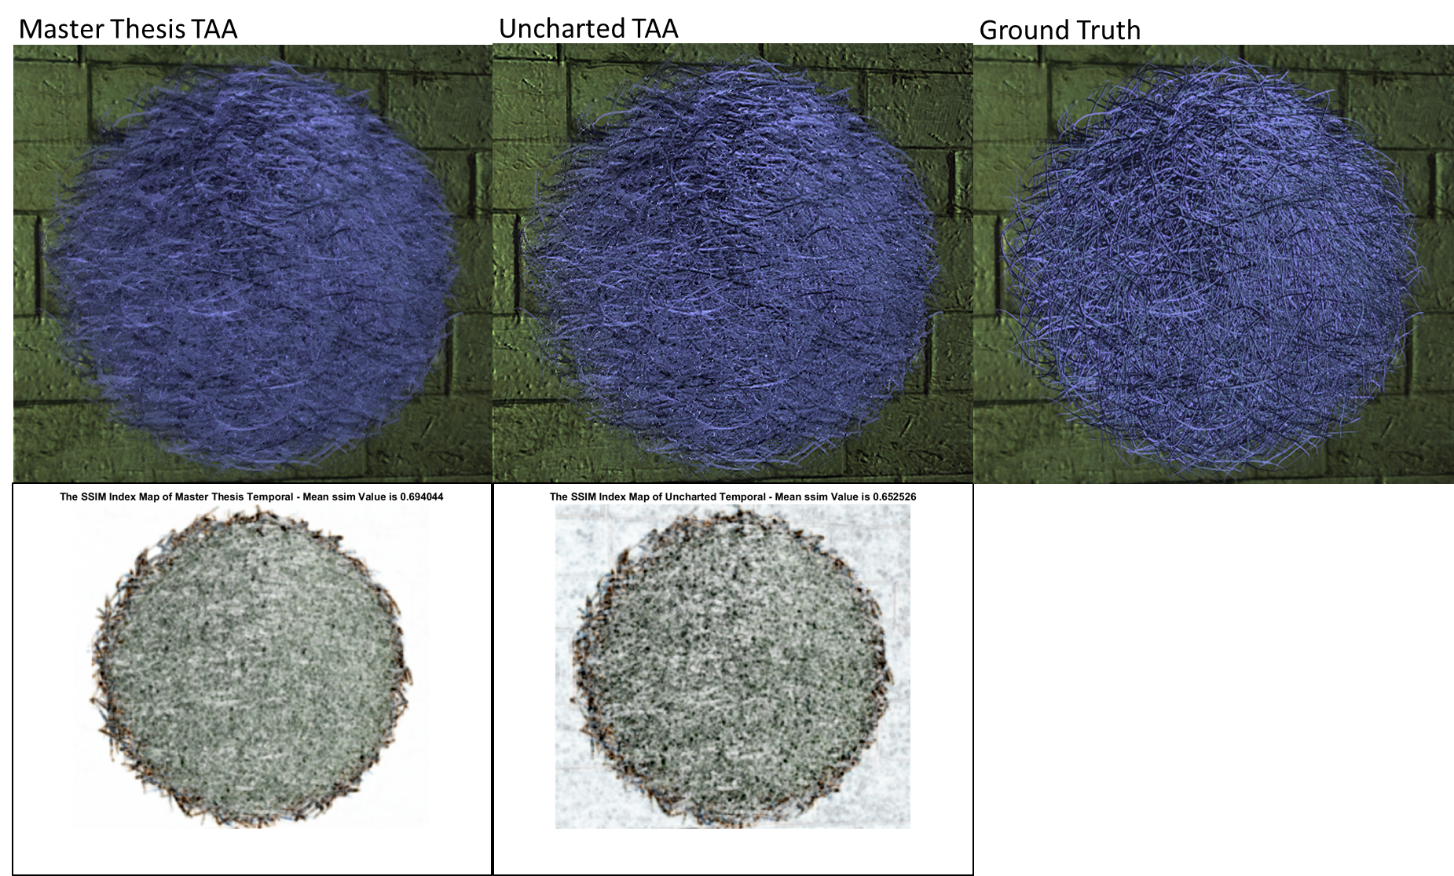
\includegraphics[scale=0.8]{images/results/hairball_ghosting_lighted.png}
	\caption{Ghosting comparison between Master Thesis TAA, Uncharted TAA and Ground Truth on Test Number 83.}\label{fig:hairball_ghosting_lighted}
\end{figure}


\subsection{Timing} \label{result_timing}
It is important to note that all the tested techniques are of Post-Processing nature, that means that they receive the output image from the Deferred Shading Architecture as input, making them not dependent on the complexity of the scene.
 
The measured time the Master Thesis TAA technique took to run was between $0.5$ and $0.6$ $ms$ on average. The Sobel pass took between $0.2$ $ms$ and $0.3$ $ms$, and the reprojection was around $0.3$ $ms$. The measured time the Uncharted TAA technique took was between $0.2$ $ms$ and $0.3$ $ms$; FXAA took between $0.1$ $ms$ and $0.2$ $ms$; and SMAA took $0.2$ $ms$ and $0.3$ $ms$.

\section{Discussion}
As we appreciate the results of the Sharpen Filter Test, see Table \ref{tab:sharpen_res}, the improvements achieved in this master thesis go beyond modifying the filter from the Uncharted implementation, because changing this filter only avoids generating those wrong bright pixels around edges. We believe that their use of that specific filter is of artistic nature. It tends to pronounce the edges at the cost of creating bright pixels around the edges that flicker, especially, when the camera moves while the foreground is illuminated but the background is on shadows or vice versa. 

From both Pipe Tests we can observe that the results from the Master Thesis TAA are close to SMAA results when drawing hard edges. We can quantify the reduction of blurring when comparing to the Uncharted TAA implementation in the numerical results from the Tables \ref{tab:pipe_regular} and \ref{tab:pipe_inclination}. When we compare the SSIM maps results (Figures \ref{fig:pipe_regular_render} and \ref{fig:pipe_inclination_render}), we observe that the thick error line around the edges in the Uncharted implementation is not present our Master Thesis implementation. But, the blurring reduction is not perfect, as we see on the tests scores, the blurring that remains around the edges lets SMAA the high score on some tests.

From the Window with Blinds and Arched Window Tests we can appreciate how the techniques react to small, almost pixel sized, features like the blinds and the doors from the Arched Window. Although the Master Thesis TAA and SMAA appear numerically (See Tables \ref{tab:window_blind} and \ref{tab:window_arch}) better than the Uncharted TAA, they are not able to reconstruct all the small details leaving pixel thin stripes that flicker when the camera moves. We believe that in this case, admitting the blurring of the Uncharted TAA benefits its final application because losing some small details is better than having many pixels flickering each time the camera moves.

The Sponza Atrium Test shows us that the Master Thesis TAA is more than capable of handling a general scene with lighting and shadows. As seen in the Table \ref{tab:sponza}, our implementation proved to be better than the other Anti-Aliasing techniques by a fair margin in almost all the tests.

We consider the Sponza Atrium Flowers Test a distinctive experiment because the flowers are a 2D flat surface with many complex transparent holes and they are rotated around the column. As we observe from the numerical results in the Table \ref{tab:sponza_flowers} and SSIM maps on Figure \ref{fig:sponza_flowers_render}, all the techniques struggle with those transparent holes but our Master Thesis TAA proves to be the best at handling them.  We see from this test that our implementation is good at handling this type of small details, compared to the Windows Tests, because they are larger than just a pixel. 

From the Hard Edges Test we continue to observe that the Master Thesis technique handles better the blur compared to the Uncharted TAA (See Table \ref{tab:hard_test}), especially on the letters, the pipe, and the square; and that the Master Thesis technique still has a hard time handling the super fine details from the windows, at this distance we still believe the blurring of the Uncharted TAA helps to hide the unwanted pixel stripes that flicker (See Figure \ref{fig:hard_test_render}).

In the Sphere Ghosting Test we see a clear example of the improvements accomplished in this Thesis. Figure \ref{fig:sphere_ghosting} shows one example of the ghosting that is created by the Uncharted TAA implementation, we can clearly perceive the stripes that are left by the sphere while it moves, whereas on our Master Thesis TAA implementation they are barely visible.

Finally, we have the four Hairball Tests, the most complex tests performed. The Hairball model has many gaps and small details that react to lighting and shadows. We anticipated a high amount of errors due to them because all Anti-Aliasing techniques have difficulties reconstructing this high density of fine details. 

On the Shadow and Light Static Test (See Tables \ref{tab:hairball_static_shadow} and \ref{tab:hairball_static_lighted}) we can observe that the Master Thesis Implementation is the best at handling the hair fibers. It is able to reconstruct smoother edges than the Uncharted TAA and reconstructs more details than SMAA technique. Especially on the light version (See Figure \ref{fig:hairball_static_lighted_render}), we can appreciate how smooth the result is; it looks almost like the ground truth. This test far exceeded the expectation of our improvements, the visual and numerical (See Table \ref{tab:hairball_static_lighted}) results shows a big increase in quality compared to the other Anti-Aliasing solutions.

On the Shadow and Light Ghosting Test we observe that both techniques results are blurred excessively (See Figures \ref{fig:hairball_ghosting_shadow} and \ref{fig:hairball_ghosting_lighted}), especially the Master Thesis TAA implementation on the light version. We believe this to be caused by the History Buffer and the Sobel Temporal Pass, for the Master Thesis TAA, not being able to stabilize as fast as the colors change when the fibers move thanks to the color rejection being slower than needed. The numerical values from Tables \ref{tab:hairball_ghosting_shadow} and \ref{tab:hairball_ghosting_lighted} confirm the effects of blurring thanks to the MSE being higher than normal.


From our timing results (See \ref{result_timing}), we can see that our improvements fit the time requirements to run on real-time applications as it is below the $1$ $ms$ common limit.


\chapter{Conclusions and Recommendations}
As we have shown numerically and visually with the tests performed, the Master Thesis implementation accomplished its objective of reducing the effects of blurring and ghosting of the Temporal Anti-Aliasing technique with the use of edge detection of both color and depth, and triangle indexing. Our results show that this technique can provide the same or better quality than other standard Anti-Aliasing solutions. 

As possible improvements, we are confident that our implementation could be optimized to run faster than our current timing. Our current implementation was made with flexibility in mind to help us test different approaches. This could be simplified to reduce the number of passes required. 

As for recommendations for further research, we suggest improving the technique's behavior under high detail density moving objects, like on the Hairball Tests. Another improvement subject is the stability for pixel size details that cause flickering, like on the Windows Tests. Furthermore, a Specular Lighting Anti-Aliasing solution compatible with Temporal Anti-Aliasing is still required to provide a full range solution to Aliasing in real-time applications. Also, we suggest searching for more specific Image Metrics for Computer Graphics, especially, finding tuning values for SSIM to provide more numerical resolution when comparing different rendered images.


\makebibliography{MyMSc}

\begin{appendices}
\chapter{GitHub Repository}
The main link to the repository is \href{https://github.com/maniatic0/Christian-TRAA}{https://github.com/maniatic0/Christian-TRAA} . From there, the next links can be accessed for the printed version of this report.
\begin{itemize}
	\item \href{https://github.com/maniatic0/Christian-TRAA}{Full Repository}.
	\item \href{https://github.com/maniatic0/Christian-TRAA/tree/master/PC\%20Specification}{Complete Computer Specification}.
	\item \href{https://github.com/maniatic0/Christian-TRAA/tree/master/Important\%20Tests}{All Tests}.
	\item \href{https://github.com/maniatic0/Christian-TRAA/tree/master/Important\%20Tests/Accumulation\%20Buffer\%20Tests}{Accumulation Buffer Tests}.
	\item \href{https://github.com/maniatic0/Christian-TRAA/tree/master/Important\%20Tests/Master\%20Thesis\%20Tests}{Most of the Master Thesis Tests}.
	\item \href{https://github.com/maniatic0/Christian-TRAA/tree/master/Important\%20Tests/Sharpening\%20Tests}{Sharpening Tests}.
	\item \href{https://github.com/maniatic0/Christian-TRAA/tree/master/Important\%20Tests/Ghosting}{Ghosting Tests}.
	\item \href{https://github.com/maniatic0/Christian-TRAA/tree/master/Important\%20Tests/HairBall}{HairBall Tests}.
	\item \href{https://github.com/maniatic0/Christian-TRAA/tree/master/CG_Labs}{Code}.
	\item \href{https://github.com/maniatic0/Christian-TRAA/tree/master/LaTeX/Master_Thesis}{\LaTeX Report}.
\end{itemize}
\chapter{Camera Jittering Explanation} \label{appendix:jitter}
The $Halton Sequence (2, 3)$ generates points in the $[0,1]\times [0,1]$ space. First, we need to transform it to the $[-1,1]\times [-1,1]$ space because we consider the pixel to be at the center, i.e. in OpenGL the first pixel is at $(0.5, 0.5)$, so we apply the transformation $T_1(x, y) = 2 * (x, y) – (1, 1)$.

Now, we only want to jitter inside the pixel because we should only be sampling inside of it. We want to control this but for explanation purposes, we can assume that we only want it inside the pixel. So, we apply the transformation $T_2(x, y) = \frac{(x, y)}{2}$.

From now on, we need to change how we interpret the process we are performing; we are calculating the distance we are going to move the pixel center, so we need to see it as a vector rather than a point. We need to transform the vector to a vector normalized by the screen size. Consequently, we apply the transformation $T_3(x, y) = (x, y) / (w, h)$ with $(w, h)$ being the Width and Height of the screen and “$/$” operator as component-wise division.

Now we need to transform our vector normalized by the screen size $[0, 1]$ to the Normalized Device Coordinates which go in the range $[-1, 1]\times [-1, 1]$. This is done by using $T_4(x, y) = 2 * (x, y)$ (to transform points we would use $2*(x, y) – (1, 1)$).
At the end, our transformation would look like this $T(x, y) = T_4(T_3(T_2(T_1(x, y)))) = (2 * (x, y) – (1, 1)) / (w, h)$ with $(x, y)$ being a Halton Sequence point.

We now need to modify our Projection Matrix, which takes points from the View Space into the Clip Space. The resulting matrix is taken from the Ke Xu presentation page 14 ~\cite{XU2016}. Let $(h_x,h_y)$ be jitter we have previously calculated.

\begin{equation}
\begin{split}
JitteredProjection = & \begin{bmatrix*} 
a & 0 & h_x & 0 \\ 
0 & b & h_y & 0 \\
0 & 0 & c & d   \\
0 & 0 & -1 & 0   \end{bmatrix*} = JitterMatrix\times Projection \\
= & \begin{bmatrix*} 
1 & 0 & 0 & -h_x \\ 
0 & 1 & 0 & -h_y \\
0 & 0 & 1 & 0   \\
0 & 0 & 0 & 1   \end{bmatrix*} \times \begin{bmatrix*} 
a & 0 & 0 & 0 \\ 
0 & b & 0 & 0 \\
0 & 0 & c & d   \\
0 & 0 & -1 & 0   \end{bmatrix*}
\end{split}
\end{equation}

Let’s see its effect to a point in View Space, let $p_{view}=(x,y,z,1)$.

\begin{equation}
	JitteredProjection\times p_{view} = \begin{bmatrix*}
	a*x+h_x*z \\
	b*y+h_y*z \\
	c*z+d \\
	-z
	\end{bmatrix*}
\end{equation}

We proceed to do the Perspective Divide to transform the point to NDC Coordinates, this is accomplished by dividing the vector by the w component.

\begin{equation}
\begin{bmatrix*}
-a*\frac{x}{z}-h_x \\
-b*\frac{y}{z}-h_y \\
-c+\frac{d}{z}d \\
1
\end{bmatrix*} = p_{NDC} + \begin{bmatrix*}
-h_x \\
-h_y \\
0 \\
0
\end{bmatrix*}
\end{equation}

Accordingly, we only need to be sure we can apply the Jitter Matrix alone to use it inside Pixel Shaders with points in NDC space. 

\begin{equation}
	JitterMatrix\times p_{NDC} = \begin{bmatrix*}
	x_{NDC}-h_x \\
	y_{NDC}-h_y \\
	z_{NDC} \\
	1
	\end{bmatrix*} = p_{NDC} + \begin{bmatrix*}
	-h_x \\
	-h_y \\
	0 \\
	0
	\end{bmatrix*}
\end{equation}

\end{appendices}


\end{document}